%% \documentclass[sigplan,preprint,screen]{acmart}\settopmatter{printfolios=true,printccs=false,printacmref=false}
\documentclass[sigplan,10pt,review,anonymous,screen]{acmart}\settopmatter{printfolios=true,printccs=false,printacmref=false}

%%
%% \BibTeX command to typeset BibTeX logo in the docs
\AtBeginDocument{%
  \providecommand\BibTeX{{%
    \normalfont B\kern-0.5em{\scshape i\kern-0.25em b}\kern-0.8em\TeX}}}

%% Copyright information
%% Supplied to authors (based on authors' rights management selection;
%% see authors.acm.org) by publisher for camera-ready submission;
%% use 'none' for review submission.
\setcopyright{none}

%%%%%%%%%% Packages
\usepackage{booktabs}
\usepackage{subcaption}
\usepackage{mathtools}
\usepackage{amsmath}
\usepackage{amssymb}
\usepackage{amsthm}
\usepackage{semantic}
\usepackage{stmaryrd}
%% \usepackage{hyperref}
%% \hypersetup{
%%   colorlinks=true,
%%   linkcolor=blue,
%% }
%% \usepackage{xcolor}
\usepackage{tikz}
\usetikzlibrary{arrows,decorations.markings}
\pgfdeclarelayer{bg} % declare background layer
\pgfsetlayers{bg,main} % set the order of the layers (main is the standard layer)

\usepackage{enumitem}
\usepackage{listings}
%% \usepackage{url}
%% \def\UrlBreaks{\do\/\do-}
%% \usepackage{wrapfig}
\usepackage{multirow}
\usepackage{hhline}
\usepackage{adjustbox}
\usepackage{ifthen}
\usepackage{colortbl}

\definecolor{mordantred19}{rgb}{0.68, 0.05, 0.0}
\definecolor{forestgreen}{rgb}{0.13, 0.55, 0.13}
\definecolor{mediumtealblue}{rgb}{0.0, 0.33, 0.71}
\definecolor{dimgray}{rgb}{0.41, 0.41, 0.41}

\colorlet{myred}{mordantred19}
\colorlet{mygreen}{forestgreen}
\colorlet{myblue}{mediumtealblue}
\colorlet{mygray}{dimgray}

\lstset{
  basicstyle=\ttfamily\footnotesize,
  columns=fullflexible,
  emph={fun, assert, Definition, Rule, rule, Endrule, endrule, using, template, accepts, holding, release, from, me, requires, transition, ltac},
  emphstyle={\bfseries\color{mygreen}},
  %% backgroundcolor=\color{backcolour},
  %% commentstyle=\color{codegreen},
  %% keywordstyle=\color{magenta},
  %% numberstyle=\tiny\color{codegray},
  %% stringstyle=\color{codepurple},
  breakatwhitespace=false,
  %% breaklines=true,
  %% captionpos=b,
  belowcaptionskip=8pt,
  keepspaces=true,
  numbers=left,
  numbersep=5pt,
  showspaces=false,
  showstringspaces=false,
  showtabs=false,
  tabsize=2,
  frame=single,
  xleftmargin=0.03\columnwidth,
  xrightmargin=0.03\columnwidth,
}
\def\slstinline{\lstinline[basicstyle=\ttfamily\small]}

\begin{document}

%% Title information
%% \title[Short Title]{Full Title}
\title{Hemiola: A Framework for Structural Design and Proof of Cache-Coherence Protocols}
%% \titlenote{}
%% \subtitle{\emph{DRAFT: please do not distribute.}}
%% \subtitlenote{}

%% \author{Joonwon Choi}
%% \author{Adam Chlipala}
%% \affiliation{
%%   \institution{MIT CSAIL}
%%   \country{USA}
%% }

\begin{abstract}
  Hardware cache-coherence protocols provide the illusion of shared memory address spaces with atomic word-level access.
  Under the hood, we often find multiple memory-access transactions executed in a distributed manner, across the levels of a cache hierarchy, and this source of concurrency is one of the greatest challenges in formal verification of cache coherence.
  We introduce \hemiola{}, a framework for designing, proving, and synthesizing cache-coherence protocols, where a central reasoning principle is provided by the framework, allowing a user to prove a specific protocol assuming that \emph{memory accesses come one-at-a-time}.
  At the framework level, using commuting reductions, we prove that any state reachable with concurrent memory access is also reachable with serialized memory access.
  The proof relies on conditions on the protocol topology and state-change rules, but we have designed a domain-specific protocol language that guides the user to design protocols that satisfy these properties by construction.
  We implemented \hemiola{} as a framework embedded in Coq and used it to design and prove hierarchical noninclusive MSI and MESI protocols as case studies.
  %% , and we synthesized these protocols to run on FPGAs.
\end{abstract}

%% Commands --

%% General commands
\newcommand{\todo}[1]{\emph{\textcolor{red}{TODO: #1}}}
\newcommand{\note}[1]{\emph{\textcolor{blue}{NOTE: #1}}}
\newcommand{\panic}[1]{\textbf{\textcolor{red}{(#1)}}}

\renewcommand{\subsectionautorefname}{section}
\renewcommand{\subsubsectionautorefname}{section}

\newcommand{\ie}{i.e.,}
\newcommand{\eg}{e.g.,}
\newcommand{\aka}{a.k.a.}

\newcommand{\tuple}[1]{\langle #1 \rangle}
\renewcommand\qedsymbol{$\blacksquare$}

%% Hemiola

\newcommand{\hemiola}{Hemiola}

\renewcommand{\listof}[1]{\ensuremath{\overline{#1}}}
%% \newcommand{\listtof}[1]{\ensuremath{\overrightarrow{#1}}}
\newcommand{\listtof}[1]{\ensuremath{\overline{#1}}}
\newcommand{\listnil}{\ensuremath{\lbrack\rbrack}}
\newcommand{\listcons}[2]{\ensuremath{#1 : #2}}
\newcommand{\listsingle}[1]{\ensuremath{\lbrack #1 \rbrack}}
\newcommand{\listapp}[2]{\ensuremath{#1 + #2}}
\newcommand{\listsub}[2]{\ensuremath{#1 - #2}}
\newcommand{\listdisj}[2]{\ensuremath{#1 \; \# \; #2}}
\newcommand{\listconcat}[1]{\ensuremath{\oplus #1}}
\newcommand{\sizeof}[1]{\ensuremath{|\, #1\, |}}

\newcommand{\mapupd}[3]{\listapp{#1}{(#2, #3)}}
\newcommand{\mapupds}[2]{\listapp{#1}{#2}}
\newcommand{\mapsubs}[2]{\listsub{#1}{#2}}

%% Stretchable squiggly arrows
%% cf. https://tex.stackexchange.com/questions/75669/how-do-i-put-text-over-a-squiggly-arrow
\newcommand{\squig}{{\scriptstyle\sim\mkern-3.9mu}}
\newcommand{\lsquigend}{{\scriptstyle\lhd\mkern-3mu}}
\newcommand{\rsquigend}{{\scriptstyle\rule{.1ex}{0ex}\rhd}}
\newcounter{sqindex}
\newcommand\squigs[1]{%
  \setcounter{sqindex}{0}%
  \whiledo {\value{sqindex}< #1}{\addtocounter{sqindex}{1}\squig}%
}
\newcommand\rsquigarrow[2]{%
  \mathbin{\stackon[2pt]{\squigs{#2}\rsquigend}{\scriptscriptstyle\text{#1\,}}}%
}
\newcommand\lsquigarrow[2]{%
  \mathbin{\stackon[2pt]{\lsquigend\squigs{#2}}{\scriptscriptstyle\text{\,#1}}}%
}

\newcommand{\idxOf}[1]{\ensuremath{#1.i}}

\newcommand{\boolt}{\ensuremath{\mathbb{B}}}
\newcommand{\propt}{\ensuremath{\mathbb{P}}}
\newcommand{\hidt}{\ensuremath{\mathbb{I}}}
\newcommand{\hidxt}{\ensuremath{\mathbb{I}}}
\newcommand{\hvaluet}{\ensuremath{\mathbb{V}}}
\newcommand{\hmsgt}{\ensuremath{\mathbb{M}}}
\newcommand{\hostt}{\ensuremath{\mathbb{O}}}
\newcommand{\hidmt}{\ensuremath{\mathbb{IM}}}
%% \newcommand{\hprect}{\ensuremath{\mathcal{P}}}
%% \newcommand{\htrst}{\ensuremath{\mathcal{T}}}

\newcommand{\hsysIn}[1]{\ensuremath{\listof{#1_{\textrm{in}}}}}
\newcommand{\hsysRq}[1]{\ensuremath{\listof{#1_{\textrm{rq}}}}}
\newcommand{\hsysRs}[1]{\ensuremath{\listof{#1_{\textrm{rs}}}}}
\newcommand{\hsys}[4]{\ensuremath{\tuple{#1, #2, #3, #4}}}
\newcommand{\hsyss}[2]{\hsys{#1}{\hsysIn{#2}}{\hsysRq{#2}}{\hsysRs{#2}}}
\newcommand{\hsysInA}[1]{\ensuremath{#1.\hsysIn{i}}}
\newcommand{\hsysRqA}[1]{\ensuremath{#1.\hsysRq{i}}}
\newcommand{\hsysRsA}[1]{\ensuremath{#1.\hsysRs{i}}}

\newcommand{\hsysobjs}[1]{\ensuremath{#1.\listof{O}}}
\newcommand{\hobjrules}[1]{\ensuremath{#1.\listof{r}}}

\newcommand{\msgbuild}[3]{\tuple{#1, #2, #3}}
\newcommand{\msgty}{\ensuremath{\textsf{ty}}}
\newcommand{\msgid}{\ensuremath{\textsf{id}}}
\newcommand{\msgval}{\ensuremath{\textsf{val}}}
\newcommand{\mtypeOf}[1]{#1.\msgty{}}
\newcommand{\midOf}[1]{#1.\msgid{}}
\newcommand{\mvalOf}[1]{#1.\msgval{}}
\newcommand{\idmbuild}[2]{\ensuremath{(#1, #2)}}

\newcommand{\ruleprec}{\ensuremath{\textsf{prec}}}
\newcommand{\ruletrs}{\ensuremath{\textsf{trs}}}
\newcommand{\rprecOf}[1]{#1.\ruleprec{}}
\newcommand{\rtrsOf}[1]{#1.\ruletrs{}}

\newcommand{\msgIns}[1]{\listof{#1^{\textrm{ins}}}}
\newcommand{\msgOuts}[1]{\listof{#1^{\textrm{outs}}}}
\newcommand{\midxIns}[1]{\listof{\idxOf{#1^{\textrm{ins}}}}}
\newcommand{\midxOuts}[1]{\listof{\idxOf{#1^{\textrm{outs}}}}}

\newcommand{\lblEmpty}{\ensuremath{l_\epsilon}}
\newcommand{\lblIns}[1]{\ensuremath{l_{\textrm{in}}(#1)}}
\newcommand{\lblOuts}[1]{\ensuremath{l_{\textrm{out}}(#1)}}
\newcommand{\lblInt}[4]{\ensuremath{l_{\textrm{int}}(#1, #2, #3, #4)}}

\newcommand{\hmpt}{\ensuremath{\mathcal{M}}}
\newcommand{\hsttr}{\ensuremath{\listtof{\hostt} \ast \hmpt}}
\newcommand{\hstt}{\ensuremath{\mathbb{S}}}
\newcommand{\hst}[2]{\ensuremath{\tuple{#1, #2}}}
\newcommand{\hstm}[2]{\ensuremath{\left\langle\begin{array}{l}#1,\\ #2 \end{array}\right\rangle}}

\newcommand{\objInit}[1]{\ensuremath{#1_{\textsf{init}}}}
\newcommand{\sysInit}[1]{\ensuremath{#1_{\textsf{init}}}}

\newcommand{\disj}[2]{\ensuremath{#1 \; \# \; #2}}
\newcommand{\nodup}[1]{\ensuremath{\textsf{nodup}\: #1}}
\newcommand{\heads}[1]{\ensuremath{#1.\textsf{hds}}}

\newcommand{\semstep}[4]{\ensuremath{#2 \xrightarrow[#1]{#3} #4}}
\newcommand{\semsteps}[4]{\ensuremath{#2 \xRightarrow[#1]{#3} #4}}
\newcommand{\semrch}[2]{\ensuremath{#1 \Rightarrow #2}}
\newcommand{\semleg}[2]{\ensuremath{#1 \xRightarrow{#2} \bullet}}
\newcommand{\sembeh}[2]{\ensuremath{#1 \Downarrow #2}}
\newcommand{\behOf}[1]{\ensuremath{\llbracket #1 \rrbracket}}

\newcommand{\refines}[2]{\ensuremath{#1 \sqsubseteq #2}}

\newcommand{\enqMsgs}[2]{\mapupds{#1}{#2}}
\newcommand{\deqMsgs}[2]{\mapsubs{#1}{#2}}

%% Serializability

\newcommand{\atomic}[3]{\ensuremath{#1 \stackrel{#2}{\squigs{3}\rsquigend} #3}}
\newcommand{\atomicLong}[4]{\ensuremath{#1 \stackrel{#2}{\squigs{#3}\rsquigend} #4}}
\newcommand{\extatomic}[4]{\ensuremath{#1 \vdash #2 \stackrel{#3}{\squigs{3}\rsquigend}_{\textsf{ext}} #4}}
\newcommand{\extatomicLong}[5]{\ensuremath{#1 \vdash #2 \stackrel{#3}{\squigs{#4}\rsquigend}_{\textsf{ext}} #5}}
\newcommand{\trsn}[2]{\ensuremath{#1 \sswarrow #2}}

\newcommand{\extatomicshort}[2]{\ensuremath{#1 \stackrel{#2}{\rightsquigarrow}_{\textsf{ext}}}}
\newcommand{\intatomicshort}[2]{\ensuremath{#1 \stackrel{#2}{\rightsquigarrow}_{\textsf{int}}}}

\newcommand{\amsgi}[1]{\ensuremath{#1^{\textrm{init}}}}
\newcommand{\amsge}[1]{\ensuremath{#1^{\textrm{end}}}}

\newcommand{\hseq}[2]{\ensuremath{\mathsf{Sequential}\ #1\ #2}}
\newcommand{\hsrzl}[2]{\ensuremath{\mathsf{Serializable}\ #1\ #2}}
\newcommand{\hsrz}[1]{\ensuremath{\mathsf{Serializable}\ #1}}

\newcommand{\strsn}[2]{\ensuremath{#1 \sswarrow_{s} #2}}
\newcommand{\hsseq}[3]{\ensuremath{#1 \parallel_{#3} #2}}

%% Visualization of messages/histories

\newcommand*\rdrecsm[1]{
  \adjustbox{raise=.1ex, trim=2.3pt 0pt 0pt 0pt}{
    \tikz[baseline=(char.base)]{
      \node[shape=rectangle, draw, inner sep=0pt, minimum size=7pt, fill=white, text=myred]
      (char) {\scriptsize\sffamily\bf #1};}}
}
\newcommand*\blrecsm[1]{
  \adjustbox{raise=.1ex, trim=2.3pt 0pt 0pt 0pt}{
    \tikz[baseline=(char.base)]{
      \node[shape=rectangle, draw, inner sep=0pt, minimum size=7pt, fill=white, text=myblue]
      (char) {\scriptsize\sffamily\bf #1};}}
}

\newcommand*\rdcircf[1]{
  \adjustbox{raise=.2ex, trim=2.3pt 0pt 0pt 0pt}{
    \tikz[baseline=(char.base)]{
      \node[shape=circle, inner sep=0pt, minimum size=8pt, fill=myred, text=white]
      (char) {\tiny\sffamily #1};}}
}
\newcommand*\blcircf[1]{
  \adjustbox{raise=.2ex, trim=2.3pt 0pt 0pt 0pt}{
    \tikz[baseline=(char.base)]{
      \node[shape=circle, inner sep=0pt, minimum size=8pt, fill=myblue, text=white]
      (char) {\tiny\sffamily #1};}}
}

\newcommand{\rdrecmsg}[2]{{\color{myred}\rdrecsm{#1}{\sf #2}}}
\newcommand{\rdrecmsgsm}[2]{\rdrecmsg{#1}{\small #2}}
\newcommand{\blrecmsg}[2]{{\color{myblue}\blrecsm{#1}{\sf #2}}}
\newcommand{\blrecmsgsm}[2]{\blrecmsg{#1}{\small #2}}

\newcommand{\msgsf}[1]{\ensuremath{\textsf{#1}}}
\newcommand{\msgsfsm}[1]{{\small\ensuremath{\textsf{#1}}}}
\newcommand{\rdmsg}[1]{{\color{myred}\msgsf{#1}}}
\newcommand{\rdmsgsm}[1]{{\color{myred}\msgsfsm{#1}}}
\newcommand{\blmsg}[1]{{\color{myblue}\msgsf{#1}}}
\newcommand{\blmsgsm}[1]{{\color{myblue}\msgsfsm{#1}}}
\newcommand{\idmsf}[2]{\idmbuild{#1}{\textsf{#2}}}
\newcommand{\spredmsg}[3]{\ensuremath{#1 \vdash #2\{#3\}}}
\newcommand{\predmsg}[2]{\ensuremath{#1\{#2\}}}

\newcommand{\rulelbl}[2]{\ensuremath{#1:(#2)}}
\newcommand{\rdrulelbl}[2]{{\small\color{myred}\rulelbl{#1}{#2}}}
\newcommand{\blrulelbl}[2]{{\small\color{myblue}\rulelbl{#1}{#2}}}

%% -- End of Commands

\maketitle

\section{Introduction}
\label{sec-intro}

\todo{Mention interleavings, noninterference lemmas used in model checking, and \hemiola{}'s contribution to establish the serializability guarantee as the most general form of the noninterference property, with a minimal set of abstract conditions that are not coupled with any specific cache-coherence protocols.}

Cache-coherence protocols have been regarded as one of the greatest correctness challenges of the hardware world.
Industry has most commonly used testing and bounded model checking for quality assurance of cache-coherence implementations, but these techniques are not sound and sometimes miss subtle bugs.%% ~\cite{ccbug}.

Research on model checking and theorem proving has produced sound techniques, though typically with significant limitations:
either the verification is of a specific protocol, or state-space-explosion concerns limit applicability to quite small cache topologies~\cite{Komuravelli:2014,Murali:2015,Banks:2017,Oswald:2018}.
In order to overcome the latter, recent approaches~\cite{Chen:2008,Chen:2010,McMillan:2016,Opeoluwa:2016,Opeoluwa:2017,Oswald:2020} utilized the notion of \emph{modularity} and successfully built verification tools that are scalable enough to verify hierarchical cache-coherence protocols.

However, these modularity disciplines impose significant restrictions in protocol design, in order to obtain clear module boundaries among caches.
A concrete limitation of modular design and verification comes when trying to verify cache-coherence protocols that are not \emph{inclusive}.
Noninclusive caches have been in common industrial use for a decade: AMD Opteron servers are known to use exclusive caches~\cite{Irazoqui:2016}, and Intel Skylake-X processors use noninclusive\footnote{Intel uses the term ``noninclusive cache'' to say that the cache is neither inclusive nor exclusive.} caches~\cite{intel-non-inclusive,Zhao:2010,Yan:2019}.

We would like to view the verification of hierarchical cache-coherence protocols from a different perspective.
Viewing a cache-coherence protocol as a global distributed protocol, we look for commonalities across well-designed protocols.
%% cross-cutting, global property that holds across all cache hierarchies.
It is a good start to identify ``good-hygiene'' properties, but it is even better to formalize such properties in frameworks that guide the design of protocols.
Then we can provide nonobvious and useful reasoning principles by-construction.

Looking for another way to factor proofs, we can find a hint in terminology often employed by protocol designers and verification engineers.
These protocols are distributed message-passing systems, so we can apply traditional software terminology like \emph{transaction} to them directly, and in fact we find similar intuitions employed in practice.
In order to describe a case where the protocol deals with two different requests passing through the same cache, for instance, a designer often says ``this cache acts like a \emph{serialization point} so the two transactions can safely \emph{interleave} with each other.''
While the notions of interleaving and serialization are already pervasive, we have found no past work trying to find a minimal set of conditions that ensure transactions are always serialized, formalizing them in a reusable framework.

In this paper, we introduce the \hemiola{} framework, embedded in the Coq proof assistant, which dramatically decreases the burden of designing and formally proving hierarchical cache-coherence protocols.
In particular, on top of the framework, hardware developers can design cache-coherence protocols without worrying about possible complex interleavings among different transactions, standing for different concurrent memory accesses.
We establish once-and-for-all that any invariant of a protocol under serialized execution is also an invariant under the interleaved executions that are necessary for good performance.

More specifically, \hemiola{} formalizes a set of message-passing distributed protocols with tree hierarchies and particular topologies of channels between nodes, with associated locks.
These protocols are defined by associating each tree node with a set of local state-transition rules that may remove messages from incoming queues and add messages to outgoing queues.
\hemiola{} exposes a domain-specific language of protocols, such that any expressible program is guaranteed to validate a \emph{serializability} property for single memory requests.
Furthermore, our framework provides a novel invariant proof method that only requires consideration of execution histories that do not interleave memory accesses -- so that almost all formal reasoning about concurrency is confined to the framework, not proofs of individual protocols.

To demonstrate usability of our framework, we provide complete correctness proofs for hierarchical, noninclusive cache-coherence protocols as case studies.
We also demonstrate that the case-study protocols are indeed hardware-synthesizable, by using a compilation/synthesis toolchain in \hemiola{}.

\paragraph{Contributions.}
To sum up, the contribution of this paper largely consists of two parts\footnote{All the code and proofs of the framework and the case studies are available in the supplementary material we provided for the paper submission.}:
\begin{itemize}
\item We discover a minimal set of topology and lock conditions that ensures \emph{serializability}, extracted from usual cache-coherence protocol designs. We then identify a domain-specific protocol language, where every protocol defined in this language ensures serializability by construction, backed up with mechanized Coq proof (\autoref{sec-hemiola-dsl}). Lastly, we formalize how serializability helps prove correctness (refinement), by using the novel notion of \emph{predicate messages} in distributed protocols.
\item Using the protocol language, we provide the complete correctness proofs of hierarchical, noninclusive MSI and MESI cache-coherence protocols (\autoref{sec-case-study}). Ours are the first complete mechanized proofs for various hierarchical noninclusive cache-coherence protocols, and as a bonus they share a large segment of reusable proofs.
%% \item We provide a toolchain to synthesize \hemiola{} protocols to run on FPGAs, and we run experiments using our case-study protocols, in order to demonstrate that they indeed run on hardware with reasonable performance.
\end{itemize}

%% \paragraph{Organization.}
%% This paper is organized as follows: we first provide a simple yet motivating example to introduce the typical concerns in designing and proving cache-coherence protocols (\autoref{sec-example}).
%% Then we formally introduce protocol transition systems as a semantic base (\autoref{sec-trs}) and the formal notion of serializability (\autoref{sec-sz-in-hemiola}) on top of them.
%% We then introduce the \hemiola{} DSL designed to ensure serializability in cache-coherence protocols (\autoref{sec-hemiola-dsl}).
%% As case studies, we prove MSI and MESI directory protocols (\autoref{sec-case-study}) and demonstrate their synthesis to hardware (\autoref{sec-synthesis}).
%% We discuss applicability and compare to related work (\autoref{sec-discussion}) and conclude with future work (\autoref{sec-conclusion}).

\section{A Motivating Example: MSI Directory Protocol with Two Caches}
\label{sec-example}

Before introducing our method for structural design and proof of cache-coherence protocols, we provide a simple yet motivating example to explain the typical challenges.
For simplicity, in this section, we will consider a protocol only \emph{a single memory location}.
We will see it is still nontrivial to design and verify a correct protocol.

The overall goal of cache coherence is, as the name suggests, to preserve coherence among multiple candidate values in a memory subsystem.
In other words, if the system is coherent, then it should behave like an atomic memory.
This behavior inclusion is formally defined as \emph{refinement}, which will be introduced in later technical sections.
The correctness of a cache-coherence protocol is sometimes shown by proving representative invariants, not talking about the relation to the desired spec.
The single-writer/multiple-read (SWMR) invariant and the data-value invariant~\cite{ccbook:2020} are the ones; in proving the refinement of a protocol these invariants (or similar ones) are required to be proven.

\tikzset{
  pics/skeleton-pcc/.style n args={3}{
    code = {
      \node at (0, 0.2) {#1};
      \node at (-1.5, -1.5) {#2};
      \node at (1.5, -1.5) {#3};
      % between P and C_1
      \draw [line width=0.2mm, <-<] (-0.6, -0.3) -- (-1.5, -1.2);
      \draw [line width=0.2mm, <-<] (-0.4, -0.3) -- (-1.3, -1.2);
      \draw [line width=0.2mm, >->] (-0.2, -0.3) -- (-1.1, -1.2);
      % between P and C_2
      \draw [line width=0.2mm, >->] (0.6, -0.3) -- (1.5, -1.2);
      \draw [line width=0.2mm, <-<] (0.4, -0.3) -- (1.3, -1.2);
      \draw [line width=0.2mm, <-<] (0.2, -0.3) -- (1.1, -1.2);
    }
  },
  skeleton-ex1/.pic = { % C_1 external
    \draw [line width=0.2mm, <-<] (-1.6, -1.8) -- (-1.6, -2.3);
    \draw [line width=0.2mm, >->] (-1.4, -1.8) -- (-1.4, -2.3);
  },
  skeleton-ex2/.pic = { % C_2 external
    \draw [line width=0.2mm, >->] (1.6, -1.8) -- (1.6, -2.3);
    \draw [line width=0.2mm, <-<] (1.4, -1.8) -- (1.4, -2.3);
  },
  skeleton-midx-e1/.pic = {
    % C_1 external
    \node at (-1.6, -2.45) {\tiny $1$};
    \node at (-1.4, -2.45) {\tiny $2$};
  },
  skeleton-midx-e2/.pic = {
    % C_2 external
    \node at (1.6, -2.45) {\tiny $10$};
    \node at (1.4, -2.45) {\tiny $9$};
  },
  skeleton-midx-pc1/.pic = {
    % between P and C_1
    \node at (-0.65, -0.15) {\tiny $3$};
    \node at (-0.45, -0.15) {\tiny $4$};
    \node at (-0.25, -0.15) {\tiny $5$};
  },
  skeleton-midx-pc2/.pic = {
    % between P and C_2
    \node at (0.65, -0.15) {\tiny $8$};
    \node at (0.45, -0.15) {\tiny $7$};
    \node at (0.25, -0.15) {\tiny $6$};
  }
}

\tikzset{
  pics/skeleton-pcce1/.style n args={3}{
    code = {
      \pic at (0, 0) {skeleton-pcc={#1}{#2}{#3}};
      \pic at (0, 0) {skeleton-ex1};
    }
  },
  pics/skeleton-pcce2/.style n args={3}{
    code = {
      \pic at (0, 0) {skeleton-pcc={#1}{#2}{#3}};
      \pic at (0, 0) {skeleton-ex2};
    }
  },
  pics/skeleton-pcce12/.style n args={3}{
    code = {
      \pic at (0, 0) {skeleton-pcc={#1}{#2}{#3}};
      \pic at (0, 0) {skeleton-ex1};
      \pic at (0, 0) {skeleton-ex2};
    }
  },
  pics/skeleton-pc/.style n args={2}{
    code = {
      \node at (0, 0) {#1};
      \node at (0, -1.5) {#2};
      % between P and C
      \draw [<-<] (-0.2, -0.3) -- (-0.2, -1.2);
      \draw [<-<] (0, -0.3) -- (0, -1.2);
      \draw [>->] (0.2, -0.3) -- (0.2, -1.2);
      % C external
      \draw [<-<] (-0.1, -1.8) -- (-0.1, -2.3);
      \draw [>->] (0.1, -1.8) -- (0.1, -2.3);
    }
  }
}

\tikzset{
  spec/.pic = {
    \node at (0, 0) {$\textrm{Spec}(v)$};
    % C_1 external
    \draw [<-<] (-0.4, -0.3) -- (-0.5, -0.8);
    \draw [>->] (-0.2, -0.3) -- (-0.3, -0.8);
    %% \node at (-0.5, -0.95) {\tiny $1$};
    %% \node at (-0.3, -0.95) {\tiny $2$};
    % C_2 external
    \draw [>->] (0.4, -0.3) -- (0.5, -0.8);
    \draw [<-<] (0.2, -0.3) -- (0.3, -0.8);
    %% \node at (0.5, -0.95) {\tiny $10$};
    %% \node at (0.3, -0.95) {\tiny $9$};
  }
}

\begin{figure}[h]
  \begin{tikzpicture}
    \pic at (0, 0) {skeleton-pcce12={$P(S, v, S_{\tuple{1, 2}})$}{$C_1(S, v)$}{$C_2(S, v)$}};
    %% \pic at (0, 0) {skeleton-midx-e1};
    %% \pic at (0, 0) {skeleton-midx-e2};
    %% \pic at (0, 0) {skeleton-midx-pc1};
    %% \pic at (0, 0) {skeleton-midx-pc2};
    \node at (2.5, -1) {$\sqsubseteq$};
    \pic at (3.7, -0.7) {spec};
  \end{tikzpicture}
  \caption{A simple MSI directory protocol and its spec}
  \vspace{-5pt}
  \label{fig-motive-1}
\end{figure}

\autoref{fig-motive-1} shows caches and communication channels for a simple directory-based MSI protocol (LHS of $\sqsubseteq$).
Since we deal with only a single memory location, the specification (RHS of $\sqsubseteq$) is a single-value ($v$) container with atomic read and write.
There are three caches ($P$, $C_1$, and $C_2$) in the implementation, and each of them has its own status (M, S, or I) and data ($v$).
A status of a cache represents a permission on its local replica.
In this MSI protocol, an object can read/write the data with the M (``modified'') status, only read with S (``shared''), and cannot read/write with I (``invalid'').
The parent $P$ additionally has a data structure called a \emph{directory} to track the statuses of the children.
For example, a directory might be $S_{\tuple{1, 2}}$, meaning that both $C_1$ and $C_2$ have S status, in some logical snapshot of state.

Objects communicate through ordered channels, shown as $(\rightarrowtail)$ in the figure.
%% where each of it has a unique index (shown as a natural number in the figure).
$C_1$ and $C_2$ have channels to receive and respond to external requests (from processor cores).
There are three types of channels between a parent and a child: a single channel for parent-to-child messages and two channels for child-to-parent requests and responses, respectively.
It is natural to wonder why two separate channels are required from a child to a parent; we will see the reason very soon.
%% Note that channels are depicted in a logical way; the actual hardware implementation may use different hardware components (\eg{} finite-capacity FIFOs or buses) that can simulate ordered channels.

\newcommand{\blackdiamond}{\raisebox{.4ex}{\ensuremath{\scriptscriptstyle\blacklozenge}}}

\begin{figure}[h]
  \centering
  \begin{tikzpicture}
    \pic at (0, 0) {skeleton-pcce12={$P(S, v, S_{\tuple{1, 2}})$}{$C_1(S, v)$}{$C_2(S, v)$}};
    % C_1 external
    %% \pic at (0, 0) {skeleton-midx-e1};
    \node[label={[label distance=-6pt,myred]left:{\rdrecmsgsm{a}{rqWr}}},color=myred] at (-1.6, -2.05) {$\bullet$};
    % C_2 external
    %% \pic at (0, 0) {skeleton-midx-e2};
    \node[label={[label distance=-6pt,myblue]left:{\blrecmsgsm{e}{rqWr}}},color=myblue] at (1.4, -2.05) {$\bullet$};
    % Between P and C_1
    %% \pic at (0, 0) {skeleton-midx-pc1};
    \node[label={[label distance=-6pt,myred]left:{\rdrecmsgsm{b}{rqM}}},color=myred] at (-1, -0.7) {$\bullet$};
    % Between P and C_2
    %% \pic at (0, 0) {skeleton-midx-pc2};
    \node[label={[label distance=-9pt,myred]below right:{\rdrecmsgsm{d}{rsI}}},color=myred] at (0.8, -0.7) {$\bullet$};
    \node[label={[label distance=-9pt,myred]above right:{\rdrecmsgsm{c}{rqI}}},color=myred] at (1, -0.7) {$\bullet$};
    \node[label={[label distance=-9pt,myblue]below left:{\blrecmsgsm{f}{rqM}}},color=myblue] at (0.6, -0.7) {$\bullet$};

    % Curves
    \draw [->,color=myred] (-2.55, -1.85) to[out=90,in=-110] node {\rdcircf{1}} (-1.95, -0.95);
    \draw [->,color=myred] (-1.9, -0.4) to[out=70,in=110,distance=1.5cm] node {\rdcircf{3}} (1.5, -0.2);
    \draw [->,color=myred] (1.9, -0.6) to[out=-40,in=-40,distance=1cm] node {\rdcircf{4}} (1.7, -1);
    \draw [->,color=myblue] (0.9, -1.8) to[out=90,in=-45] node {\blcircf{2}} (0.3, -1.2);

    % Legends
    %% \draw [->] (2, 0) to (3, 0);
    %% \node at (2, 0) {\rdcircf{1}};
    %% \node at (2.3, 0) {\rdcircf{3}};
    %% \node at (2.6, 0) {\rdcircf{4}};
    %% \node at (2, -0.3) {\blcircf{2}};
  \end{tikzpicture}
  \caption{Rule-execution cases in the simple MSI protocol}
  \vspace{-5pt}
  \label{fig-motive-2}
\end{figure}

\autoref{fig-motive-2} depicts some example state-transition cases depending on statuses of the caches.
All the caches run concurrently, repeatedly executing \emph{rules} that define local state transitions.
A rule may take some messages from input channels, perform a state transition, and put messages in output channels.
A rule may also have a precondition, blocking use of that rule when the precondition does not hold.
\rdcircf{1} shows the case where a child $C_1$ takes an external request (\rdrecmsgsm{a}{rqWr}) to write data, but it does not have M status and thus further requests to the parent (\rdrecmsgsm{b}{rqM}) to get the permission.
At this moment, in many cache-coherence protocol designs, $C_1$ changes its status to a \emph{transient state} SM to record its current status (S) and the next expected status (M).
This transient state also functions as a \emph{lock} not to allow any further external requests for the value.

Due to the concurrent execution of the caches, we might have another rule executed at the same time.
\blcircf{2} is executed concurrently with \rdcircf{1}, where $C_2$ also takes an external request (\blrecmsgsm{e}{rqWr}) with the same purpose, thus requests \blrecmsgsm{f}{rqM} to the parent as well.
Since \rdcircf{1} and \blcircf{2} happened at the same time, now the parent $P$ needs to decide which request to deal with.
Suppose that it decided to handle \rdrecmsgsm{b}{rqM} first.

\rdcircf{3} presents the next execution by $P$, taking the input message \rdrecmsgsm{b}{rqM} and making an \emph{invalidation} request (\rdrecmsgsm{c}{rqI}) to the other child $C_2$ to change its status to I.
This invalidation request is required, since when a child has M the others should not be able to read/write the data.
The parent, at this moment, changes its directory status to a transient state (named $S^D$ in some textbooks) to disallow any other requests from the children.
For instance, the parent should not handle \blrecmsgsm{f}{rqM}, since otherwise it will handle two ``\msgsf{rqM}''s simultaneously, which might lead to an incoherent state -- two M statuses in the caches.

Lastly, \rdcircf{4} shows the case that $C_2$ handles the invalidation request (\rdrecmsgsm{c}{rqI}).
A number of corner cases should be handled carefully in this case:
\begin{itemize}[leftmargin=*]
\item Since $C_2$ requested \blrecmsgsm{f}{rqM}, it has a transient state SM when \rdrecmsgsm{c}{rqI} arrives. It should still be able to handle this invalidation request even in the transient state (while not allowing any external requests). In this case $C_2$ accepts \rdrecmsgsm{c}{rqI} and changes its transient state to IM. We see that transient states should be fine-grained enough to distinguish which requests to handle.
\item Due to the existence of \blrecmsgsm{f}{rqM}, if we had a single channel from a child to a parent, a deadlock would occur. $P$ cannot take \blrecmsgsm{f}{rqM} since it has been locked (in a transient state) after making an invalidation request. It cannot take \rdrecmsgsm{d}{rsI} as well since the response is not the first one of the ordered channel. This case shows the necessity of having multiple channels between a child and a parent.
\end{itemize}

A so-called three-channel system has been widely used and regarded as a good choice to make the design correct and live~\cite{Murali:2015,thesis:Murali:2016}.
While there are other possible correct topology and network settings, the cases shown in \autoref{fig-motive-2} at least demonstrate that it is nontrivial to construct one of them.

Transient states and network channels play a crucial role in making \emph{interleavings} correct.
Regarding the sequence of rule executions (in red) $[\rdcircf{1}; \rdcircf{3}; \rdcircf{4}]$ as an execution flow -- we will call it a \emph{transaction} in later sections -- to handle the original external request \rdrecmsgsm{a}{rqWr}, we see that no further executions could not happen after \blcircf{2}, which is for the other request \blrecmsgsm{e}{rqWr}.
As explained above case-by-case, proper transient states and network channels block \blrecmsgsm{f}{rqM} to be further proceeded.
This mechanism to ensure safe interleavings is called \emph{noninterference}, which ensures that no other state transitions affect while handling a certain transaction.
In model-checking cache-coherence protocols, lots of good noninterference lemmas have been developed and used to avoid state explosion by interleaving transactions.

While the same concern occurs in interactive theorem proving (by requiring manual proof effort to deal with interleavings), we would like to make use of a conventional advantage of interactive theorem provers: to state and prove an once-and-for-all property and to use it multiple times.
Particularly, in proving cache-coherence protocols, we want to find minimal conditions that ensures safe interleavings, \emph{extracted and abstracted} from the transient states and network channels, so the conditions can apply to multiple protocols.
Building it from the scratch, it will be required to formalize the meaning of safe interleavings first, and then to show how this formalization ease the verification of cache-coherence protocols in theorem proving.
That is exactly what we did with \hemiola{}.
In later sections, we will first see an underlying semantic model for protocols (\autoref{sec-trs}) and a formal notion of safe interleavings (called serializability) within it (\autoref{sec-sz-in-hemiola}).
We will also explain how the serializability ease the burden of verification (\autoref{sec-atomic-invariants}) and show its definite use cases in verifying our case-study protocols (\autoref{sec-case-study}).

\section{Protocol Transition Systems}
\label{sec-trs}

\paragraph{Notations.}
Throughout this paper, we will use several notations for lists (sequences) and finite maps.
An overline (\eg{} $\listof{l}$) denotes a list.
$\listnil{}$, $(\listcons{h}{\listof{t}})$, $(\listapp{\listof{l_1}}{\listof{l_2}})$, $(\listsub{\listof{l_1}}{\listof{l_2}})$, and
$(\listdisj{\listof{l_1}}{\listof{l_2}})$ denote nil, cons, append, subtraction, and disjointness of lists, respectively.
$\listconcat{\listof{l}}$ flattens the list of lists $\listof{l}$ with repeated concatenation.
$\sizeof{\listof{l}}$ is the length of a list.
Regarding a list of key-value pairs as a finite map, we override notations for lists.
For example, $(\mapupds{M}{\listof{l}})$ updates multiple key-value pairs in a finite map $M$.
Moreover, we overload the same operation $(\mapupd{M}{k}{v})$ for a single update for simplicity.
We will use $\tuple{\cdot}$ to denote a struct and use a name (\eg{} $s.\textsf{fd}$) to access a field value.
$(\listof{s.\textsf{fd}})$ will be used as a shorter notation for $(\textsf{map}\ (\lambda s.\; s.\textsf{fd})\ \listof{s})$.

\subsection{Syntax}
\label{sec-syntax}

\begin{figure}[t]
  \centering\small
  \setlength{\tabcolsep}{0pt}
  \def\arraystretch{1.1}
  \begin{tabular}{|c|}
    \hline
    \begin{math}
      \begin{array}{rl}
        \textrm{Id} & \msgid{} \in \hidxt{} \\
        \textrm{Value} & \msgval{} \in \hvaluet{} \\
        \textrm{Message} & m ::= \msgbuild{\msgty}{\msgid}{\msgval} \in \hmsgt{} \triangleq \boolt \ast \hidxt \ast \hvaluet \\
        \textrm{Index} & i \in \hidxt{}\ \textrm{(for channels, objects, etc.)} \\
        \textrm{Channel Index \& Message} & im ::= \idmbuild{i}{m} \in \hidmt \triangleq \hidxt \ast \hmsgt \\
        \textrm{Object state} & o \in \hostt{} \\
        \textrm{Rule precondition} & \ruleprec{} \in \hostt \to \listtof{\hidmt} \to \propt \\
        \textrm{Rule transition} & \ruletrs{} \in \hostt \to \listtof{\hidmt} \to \hostt \ast \listtof{\hidmt}\\
      \end{array}
    \end{math}\\
    \mbox{}\vspace{-10pt} \\ %% padding
    \hline
    \mbox{}\vspace{-10pt} \\ %% padding
    \begin{math}
      \begin{array}{rl}
        \textrm{Rule} & r ::= \tuple{i, \ruleprec{}, \ruletrs{}} \\
        \textrm{Object} & O ::= \tuple{i, \objInit{o}, \listof{r}} \\
        \textrm{System} & S ::= \hsyss{\listof{O}}{i} \\
      \end{array}
    \end{math}\\
    \hline
  \end{tabular}
  \caption{Protocol transition system}
  \label{fig-trs-system}
\end{figure}

\begin{figure*}[t]
  \small\centering
  \def\arraystretch{1.1}
  \arraycolsep=1pt
  \begin{tabular}{|c|c|}
    \hline
    \begin{tabular}{c}
      \multicolumn{1}{l}{\textbf{* Types}} \\
      \begin{tabular}{ll}
        $\textrm{Message States}\ \ M \in \hidxt{} \to \listtof{\hmsgt}$ &
        $\textrm{State}\ \ s \in \hstt{} ::= \tuple{\listof{o}, M}$ \\
        \multicolumn{2}{l}{$\textrm{Label}\ \ l ::= \lblEmpty{}\; |\; \lblIns{\listof{im}}\; |\; \lblOuts{\listof{im}}\; |\; \lblInt{\idxOf{O}}{\idxOf{r}}{\listof{im}}{\listof{im}}$} \\
      \end{tabular}\\
      \multicolumn{1}{l}{\textbf{(a) Step:}} \\
      \begin{math}
        \begin{array}{c}
          \inference[StepSilent:]{}{\semstep{S}{s}{\lblEmpty{}}{s}} \\
          \mbox{}\vspace{-5pt} \\ %% padding
          \inference[StepIns:]{\listof{im} \neq \listnil
            & \listof{\idxOf{im}} \subseteq \hsysRqA{S}}{\semstep{S}
            {\hst{\listof{o}}{M}}
            {\lblIns{\listof{im}}}
            {\hst{\listof{o}}{\enqMsgs{M}{\listof{im}}}}} \\
          \mbox{}\vspace{-5pt} \\ %% padding
          \inference[StepOuts:]{\listof{im} \neq \listnil
            & \listof{im} \subseteq \heads{M}
            & \listof{\idxOf{im}} \subseteq \hsysRsA{S}}{\semstep{S}
            {\hst{\listof{o}}{M}}
            {\lblOuts{\listof{im}}}
            {\hst{\listof{o}}{\deqMsgs{M}{\listof{im}}}}} \\
          \mbox{}\vspace{-5pt} \\ %% padding
          \inference[StepInt:]{S = \hsyss{\listof{O}}{i}
            & O \in S.\listof{O}
            & r \in O.\listof{r} \\
            \midxIns{im} \subseteq \hsysInA{S} \cup \hsysRqA{S}
            & \listof{o}[\idxOf{O}] = o_1
            & \msgIns{im} \subseteq \heads{M} \\
            r.p\enspace o_1\ \msgIns{im}
            & r.t\ o_1\ \msgIns{im} = (o_2, \msgOuts{im}) \\
            \midxOuts{im} \subseteq \hsysInA{S} \cup \hsysRsA{S}
            & \disj{\midxIns{im}}{\midxOuts{im}}}{\semstep{S}
            {\hst{\listof{o}}{M}}
            {\lblInt{\idxOf{O}}{\idxOf{r}}{\msgIns{im}}{\msgOuts{im}}}
            {\hstm{\mapupd{\listof{o}}{\idxOf{O}}{o_2}}{\enqMsgs{\deqMsgs{M}{\msgIns{im}}}{\msgOuts{im}}}}} \\
          \mbox{}\vspace{-5pt} \\ %% padding
        \end{array}
      \end{math}
    \end{tabular} &
    \begin{tabular}{c}
      \multicolumn{1}{l}{\textbf{(b) Steps and behaviors:}} \\
      \begin{math}
        \arraycolsep=5pt
        \begin{array}{cc}
          \inference[StepsNil:]{}{\semsteps{S}{s}{\listnil{}}{s}}
          & \inference[StepsCons:]{\semsteps{S}{s_0}{\listof{l}}{s_1}
            & \semstep{S}{s_1}{l_1}{s_2}}{\semsteps{S}{s_0}{\listcons{l_1}{\listof{l}}}{s_2}} \\
          \multicolumn{2}{c}{\inference[Behavior:]{\semsteps{S}{\sysInit{S}}{\listof{l}}{s}}{\sembeh{S}{\behOf{\listof{l}}}}} \\
          \mbox{}\vspace{-5pt} \\ %% padding
        \end{array}
      \end{math}\\
      \hline
      \multicolumn{1}{l}{\textbf{(c) Atomic histories:}} \\
      \begin{math}
        \begin{array}{c}
          \inference[AtomicStart:]{}{\atomicLong{\listof{\amsgi{im}}}{\listsingle{\lblInt{\idxOf{O}}{\idxOf{r}}{\listof{\amsgi{im}}}{\listof{\amsge{im}}}}}{28}{\listof{\amsge{im}}}}\\[15pt]
          \inference[AtomicCont:]{\atomic{\listof{\amsgi{im}}}{\listof{l}}{\listof{\amsge{im}}}
            & \msgIns{n} \neq \listnil
            & \msgIns{n} \subseteq \listof{\amsge{im}}}{\atomicLong{\listof{\amsgi{im}}}{\listcons{\lblInt{\idxOf{O}}{\idxOf{r}}{\msgIns{n}}{\msgOuts{n}}}{\listof{l}}}{28}{(\listapp{\listsub{\listof{\amsge{im}}}{\msgIns{n}}}{\msgOuts{n}}})} \\
          \mbox{}\vspace{-5pt} %% padding
        \end{array}
      \end{math}\\
      \hline
      \multicolumn{1}{l}{\textbf{(d) Transactions:}} \\
      \begin{math}
        \arraycolsep=5pt
        \begin{array}{cc}
          \begin{array}{c}
            \inference[TrsSilent:]{}{\trsn{S}{\listsingle{\lblEmpty{}}}} \\[5pt]
            \inference[TrsIns:]{}{\trsn{S}{\listsingle{\lblIns{\listof{im}}}}} \\[5pt]
            \inference[TrsOuts:]{}{\trsn{S}{\listsingle{\lblOuts{\listof{im}}}}} \\[5pt]
            \mbox{}\vspace{-5pt} %% padding
          \end{array} &
          \begin{array}{l}
            \textrm{\footnotesize TrsAtomic:} \\
            \inference[]{\extatomic{S}{\listof{\amsgi{im}}}{\listof{l}}{\listof{\amsge{im}}}}{\trsn{S}{\listof{l}}}
          \end{array} \\
        \end{array}
      \end{math}\\
    \end{tabular}\\
    \hline
  \end{tabular}
  \caption{Steps, behaviors, atomic histories, and transactions in protocol transition systems}
  \label{fig-trs-semantics}
\end{figure*}

\hemiola{} uses formal protocol transition systems as an underlying basis for reasoning cache-coherence protocols.
\autoref{fig-trs-system} explains what such systems are, in the style of automata theory.
A \emph{message} $m$ consists of a boolean message type (request or response), a message id (effectively from an enumeration of message kinds), and value.
A \emph{value} refers to a general set of values, principally those that can be stored at memory addresses.
A struct sometimes has an \emph{index} to distinguish it from the other components.
A pair \idmbuild{i}{m} is used to represent a message $m$ residing in a channel with an index $i$.

A rule $r$ a struct composed of its rule index (unique within an object), a precondition (\ruleprec{}), and a transition function (\ruletrs{}).
A precondition takes two arguments, a current object state and input messages, and decides whether the rule can be executed or not.
A transition function takes the same arguments but returns the next object state and a list of (channel index, message) pairs as output messages.
Our definition is shallowly embedded in Coq, \eg{} precondition and transition definitions use native Coq function types.

An object $O$ contains its object index (unique within a system), an initial state ($\objInit{o}$), and rules (\listof{r}) that make local state transitions within the object.
A system $S$ contains information about objects and channels.
It consists of objects (\listof{O}) and channel indices for internal messages (\hsysIn{i}), external inputs (\hsysRq{i}), and external outputs (\hsysRs{i}).
The definition is general in that any object can access any channel in the system, just by mentioning the channel index in a state transition.
It is necessary to distinguish between internal and external channels, in order to define external behaviors of the system.

\subsection{Semantics}
\label{sec-semantics}

\paragraph{Steps.}
\autoref{fig-trs-semantics} describes the semantics of protocol transition systems.
A state transition (step) happens by a rule that takes input messages and generates output messages.
The semantics for a step is presented as a judgment $\semstep{S}{s_0}{l}{s_1}$, where $S$ is the system to execute, $s_0$ is a prestate, $s_1$ is a poststate, and $l$ is a label generated by the state transition.
The state of a system (in domain $\hstt{}$) is a pair, consisting of object states and message states.
Object states are represented in a finite map from object indices to object states, and message states are represented in a finite map from channel indices to ordered queues of messages.

Rule [StepSilent] represents the case where no state transition happens in the current step; an empty label (\lblEmpty{}) is generated in this case.
From now on, we assume that all the input/output messages used in the step definitions do not share the same channel, \ie{} $(\nodup{\listof{\idxOf{im}}})$.
A system may accept input messages from the external world; [StepIns] describes this case, where the external input messages (\listof{im}) should not be empty, channels of the messages are valid; an external inputs label $(\lblIns{\listof{im}})$ is generated in this case.
[StepOuts] describes the opposite case, for output messages being released to the external world.
In this case, each output message should be in the head of its residing channel ($\listof{im} \subseteq \heads{M}$).

Lastly, [StepInt] deals with a state transition by a rule ($r$) in an object ($O$).
It nondeterministically chooses an object and a rule in the object, checks that the precondition holds, and applies the transition to update the state of the system; an internal label ($\lblInt{\idxOf{O}}{\idxOf{r}}{\msgIns{im}}{\msgOuts{im}}$) is generated in this case, which records an object index, a rule index, input messages, and output messages.

Note that the semantics is based on ordered channels, so messages are \emph{enqueued} and \emph{dequeued} in each state-transition case.
We use notations $\enqMsgs{M}{\listof{im}}$ and $\deqMsgs{M}{\listof{im}}$ for such operations.
It is also required that any state transition does not both dequeue and enqueue an element from the same queue; $\disj{\midxIns{im}}{\midxOuts{im}}$ in [StepInt] exactly describes this condition.

The step semantics is naturally lifted to one for multiple steps, presented as a judgment $\semsteps{S}{s_0}{\listof{l}}{s_1}$, where $S$, $s_0$, and $s_1$ are similar to ones in the step semantics, and $\listof{l}$ is a sequence of labels generated by executions of the steps.
[StepsNil] serves the case where no state transitions happen at all.
[StepsCons] is a natural inductive constructor that combines previous steps and a new one.
Note that the latest label is added to the head, thus the last label in the sequence is the oldest one.
(We found this convention convenient in Coq for usual reasons of functional-programming naturalness, and we stick with it in the paper version of the formalism to avoid transcription errors.)

We will sometimes call a sequence of labels a \emph{history}.
We say that a state $s$ is \emph{reachable} iff there is a history $\listof{l}$ such that $\semsteps{S}{\sysInit{S}}{\listof{l}}{s}$ holds, where $\sysInit{S}$ is the initial state of the system $S$, constructed by composing all initial object states.
We use a simpler notation $\semrch{S}{s}$ for reachable states.
We also say that a history $\listof{l}$ is \emph{legal} iff there is a state $s$ such that $\semsteps{S}{\sysInit{S}}{\listof{l}}{s}$ holds.
We write $\semleg{S}{\listof{l}}$ to assert that a history is legal.

It is worth noting that we take for granted that rules are executed atomically, even when multiple rules are executed at the same time.
Here we appeal to a tradition of hardware-description approaches that guarantee rule-level serialization (also known as ``one-rule-at-a-time semantics'') for this kind of design~\cite{fesi,kami,Murali:2015,Dave:2005,Dave:2007}.

\paragraph{Behaviors and correctness.}
A system $S$ has a behavior $\behOf{\listof{l}}$ (denoted as \sembeh{S}{\behOf{\listof{l}}}) if there exists an execution of steps that generates $\listof{l}$, starting with the initial state of $S$ ([Behavior]).
Here the $\behOf{\cdot}$ operation filters out silent ($l_\epsilon$) and internal ($l_{\textrm{int}}$) labels so only the external parts remain.
We call such a sequence of labels a \emph{trace}.
Finally we define a notion of correctness in \hemiola{}.
\begin{definition}[Trace Refinement]
  A system $I$ (``implementation'') trace-refines another system $S$ (``specification''), written as $\refines{I}{S}$, iff every trace of $I$ is also a trace of $S$:
  \begin{displaymath}
    \refines{I}{S} \triangleq \forall \listof{t}.\; \sembeh{I}{\listof{t}} \to \sembeh{S}{\listof{t}}.
  \end{displaymath}
\end{definition}

Trace refinement is usually proven by establishing a \emph{simulation} relation between the implementation and the spec states.
\begin{definition}[Simulation]
  We call $(\sim): \hstt{} \to \hstt{} \to \propt{}$ a simulation between the systems $I$ and $S$ iff a step in $S$ exists for every step in $I$, which generates the same external label and preserves the relation:
  \begin{align*}
    \forall s_0, s_1, l.\; & \semstep{I}{s_0}{l}{s_1} \to \forall t_0.\; s_0 \sim t_0 \to\\
    & \exists t_1.\; \semstep{S}{t_0}{l}{t_1} \wedge s_1 \sim t_1.
  \end{align*}
\end{definition}
\begin{theorem}[Simulation implies trace refinement]
  If there is a simulation $(\sim)$ between two given systems $I$ and $S$, then \refines{I}{S}.
\end{theorem}
\begin{proof}
  By the induction on state-transition steps.
\end{proof}

\section{Serializability in Protocol Transition Systems}
\label{sec-sz-in-hemiola}

Serializability~\cite{sz1,sz2} is a celebrated notion of concurrency correctness that originated with databases and distributed systems.
While each transaction in a system affects multiple values, serializability guarantees that concurrent execution of such transactions is correct in that the effect (state change) is the same as if the transactions were executed serially, \ie{} \emph{atomically in some order with no interleaving}.

In this section, we provide the formal definition of serializability and explain how it eases the burden of designing and proving conventional invariants.
It is worth recalling at this moment that we build the framework to prove cache-coherence protocols more easily.
In the next section we will explore which conditions in cache-coherence protocols ensure serializability and how to prove it with the conditions.

\subsection{From Atomic Histories to Serializability}

\subsubsection{Atomic histories}
In order to define serializability formally, we first provide basic definitions of atomic histories and transactions, presented in \autoref{fig-trs-semantics}.
A history $h$ is \emph{atomic} iff it satisfies the predicate $(\atomic{\listof{\amsgi{im}}}{h}{\listof{\amsge{im}}})$ with \emph{initial messages} $\listof{\amsgi{im}}$ and \emph{live messages} $\listof{\amsge{im}}$.
[AtomicStart] initializes a history with an internal label.
[AtomicCont] inductively adds a label to an atomic history, where the input messages of the new label \emph{should be from the live messages of the previous atomic history}.

\begin{figure}[h]
  \begin{tabular}{c}
    \begin{tikzpicture}
      \pic at (0, 0) {skeleton-pcce1={$P$}{$C_1$}{$C_2$}};
      % C_1 external
      \pic at (0, 0) {skeleton-midx-e1};
      \node[label={[label distance=-6pt,myred]left:{\sf\small rqWr}},color=myred] at (-1.6, -2.05) {$\bullet$};
      % Between P and C_1
      \pic at (0, 0) {skeleton-midx-pc1};
      \node[label={[label distance=-6pt,myred]left:{\sf\small rqM}},color=myred] at (-1, -0.7) {$\bullet$};
      % Between P and C_2
      \pic at (0, 0) {skeleton-midx-pc2};
      \node[label={[label distance=-9pt,myred]below left:{\sf\small rsI}},color=myred] at (0.8, -0.7) {$\bullet$};
      \node[label={[label distance=-9pt,myred]above right:{\sf\small rqI}},color=myred] at (1, -0.7) {$\bullet$};

      % Curves
      \draw [->,color=myred] (-2.2, -1.85) to[out=90,in=-110] node[left=3pt] {$r_1$} (-1.6, -0.95);
      \draw [->,color=myred] (-1.6, -0.45) to[out=70,in=120,distance=1.3cm] node[above] {$r_2$} (1.3, -0.2);
      \draw [->,color=myred] (1.45, -0.7) to[out=-50,in=-50,distance=1.7cm] node[below] {$r_3$} (0.5, -1.2);
    \end{tikzpicture}\\
    \hline
    \begin{math}
      \small
      \begin{array}{rl}
        h \triangleq & [\lblInt{\idxOf{C_2}}{\idxOf{r_3}}{\listsingle{(8, {\sf rqI})}}{\listsingle{(7, {\sf rsI})}};\\
          & \lblInt{\idxOf{P}}{\idxOf{r_2}}{\listsingle{(3, {\sf rqM})}}{\listsingle{(8, {\sf rqI})}};\\
          & \lblInt{\idxOf{C_1}}{\idxOf{r_1}}{\listsingle{(1, {\sf rqWr})}}{\listsingle{(3, {\sf rqM})}}]\\
      \end{array}
    \end{math}
  \end{tabular}
  \caption{An example of an atomic history}
  \vspace{-5pt}
  \label{fig-ex-atomic-history}
\end{figure}

\autoref{fig-ex-atomic-history} presents an example of an atomic history.
$h$ is generated by executions of three rules, $r_1 \in \hobjrules{C_1}$, $r_2 \in \hobjrules{P}$, and $r_3 \in \hobjrules{C_2}$.
Rule $r_1$ takes an input message $(1, \textsf{rqWr})$ (from the channel with index $1$) as an initial message of the history.
Rule $r_2$ takes $(3, \textsf{rqM})$, the output message from $r_1$.
Finally, $r_3$ takes $(7, \textsf{rqI})$, the output message from $r_2$.
Summing up all the rule executions, by the definition of an atomic history we get the predicate $\atomic{\listsingle{(1,\textsf{rqWr})}}{h}{\listsingle{(7,\textsf{rsI})}}$.
This example shows that an atomic history intuitively captures a \emph{transaction flow} triggered by the initial messages.
Note that an atomic history does not need to be a completed transaction.
The history $h$ in the example is not completed, in the sense that the live message ($\textsf{rsI}$) is not a response to an external channel.

We call a history \emph{externally atomic} if initial messages are external requests ($\listof{\idxOf{\amsgi{m}}} \subseteq \hsysRqA{S}$); we denote it as $(\extatomic{S}{\listof{\amsgi{im}}}{\listof{l}}{\listof{\amsge{im}}})$.
An externally atomic history records the way the system responded to some set of messages received from the outside world.

\subsubsection{Transactions}
Transactions are the next level of abstraction, defined by the final rules in \autoref{fig-trs-semantics}.
A transaction is either a single silent label ([TrsSilent]), a single external inputs label ([TrsIns]), a single external outputs label ([TrsOuts]), or an externally atomic history ([TrsAtomic]).
In other words, the permitted atomic execution steps, in this transactional semantics, are arrival of new messages from the outside world, release of messages to the outside world, or uninterrupted execution of an atomic history.
We denote by $\trsn{S}{h}$ that $h$ is a transaction in $S$.

Note that an external-inputs label and an atomic history are regarded as separate transactions; this relaxed design choice is due to our eventual goal, trace refinement.
In order to prove trace refinement, we should preserve the \emph{order of external labels} while reasoning over histories.
In particular, we do not want a serialized history having a different trace from the original history.
A key soundness proof of \hemiola{} will reason with reorderings of internal steps and thus atomic histories, but we will leave external labels untouched, manifestly preserving trace orders.

\subsubsection{Sequential histories and serializability}
With a clear notion of transactions, we can easily define sequential histories and serializability.

\begin{definition}[Sequential Histories and Serializability]\mbox{}\vspace{-8pt}\\
  \begin{enumerate}[leftmargin=*]
  \item A history $h$ is \emph{sequential} iff the history is a concatenation of transactions:
    \begin{displaymath}
      \hseq{S}{h} \triangleq \exists\, \listof{t}.\; (\forall t \in \listof{t}.\; \trsn{S}{t}) \wedge h = \listconcat{\listof{t}}.
    \end{displaymath}
  \item A legal history $h$ is \emph{serializable} in the system $S$ iff there exists a sequential history that reaches the same state:
    \begin{align*}
      \hsrzl{S}{h} \triangleq\; & \forall s.\; \semsteps{S}{\sysInit{S}}{h}{s} \to\\
      & \exists\, h_{\textrm{seq}}.\; \hseq{S}{h_{\textrm{seq}}} \wedge \semsteps{S}{\sysInit{S}}{h_{\textrm{seq}}}{s}.
    \end{align*}
  \item A system $S$ is \emph{serializable} iff every legal history is serializable:
    \begin{displaymath}
      \hsrz{S} \triangleq \forall h.\; \hsrzl{S}{h}.
    \end{displaymath}
  \end{enumerate}
  \label{def-sz}
\end{definition}

\subsection{The Payoff: Predicate Messages in Atomic Histories}
\label{sec-pred-msg}

Now we discuss how to exploit our notion of serializability: how does it help prove trace refinement between an implementation and its spec?
There is a clear gap between two notions, serializability and trace refinement: the former only deals with \emph{reachable states}, whereas the latter only deals with \emph{behaviors}.
However, we can bridge the gap by using serializability to help prove \emph{invariants} (which only concern reachable states), since a simulation -- which implies trace refinement -- proof usually requires a number of invariants of the implementation.

We call $\mathcal{I}: \hstt{} \to \propt{}$ an \emph{invariant} over a system $S$ if $\mathcal{I}$ holds for all reachable states, \ie{} $\forall s.\; \semrch{S}{s} \to \mathcal{I}\ s$.
In proving the correctness of a distributed protocol, it is quite common to state an invariant like ``what is the desired property if the system currently has a certain message in a certain channel?''
We call such an invariant a \emph{predicate message}, formally defined as following:
\begin{displaymath}
  \spredmsg{S}{im}{P} \triangleq \forall s.\; \semrch{S}{s} \to im \in s.M \to P\; s.
\end{displaymath}
We will just use \predmsg{im}{P} when the system $S$ is easily inferred by the context.
Sometimes even a shorter version \predmsg{\msgid{}}{P} (the one for the message with \msgid{}) will be used with clear context.

\begin{figure}[h]
  \centering
  \begin{tikzpicture}
    \pic at (0, 0) {skeleton-pcce1={$P$}{$C_1$}{$C_2$}};
    % C_1 external
    \pic at (0, 0) {skeleton-midx-e1};
    \node[label={[label distance=-6pt,myred]right:{\msgsfsm{rsWr}}},color=myred] at (-1.4, -2.05) {$\bullet$};
    % Between P and C_1
    \pic at (0, 0) {skeleton-midx-pc1};
    \node[label={[label distance=-9pt,myred]below right:{\msgsfsm{rsM}}},color=myred] at (-0.6, -0.7) {$\bullet$};
    % Between P and C_2
    \pic at (0, 0) {skeleton-midx-pc2};
    \node[label={[label distance=-6pt,myblue]right:{\small\predmsg{\msgsf{rsM}}{C_1.\textrm{st} = I \wedge P.\textrm{st} = I}??}},color=myblue] at (1, -0.7) {$\bullet$};

    % Curves
    \draw [->,color=myred] (-0.6, -1.15) to[out=225,in=90] node[below right=-3pt] {\rdrulelbl{r_1}{C_1.\textrm{st} \leftarrow M}} (-1.2, -1.85);

    % Legends
    \draw (2.3, -1.4) rectangle (5.0, -2.0) node[pos=.5]
          {\small $O.\textrm{st} \triangleq (s.\listof{o})[\idxOf{O}].\textrm{st}$};
  \end{tikzpicture}
  \caption{A predicate message becomes broken when interfered}
  \vspace{-5pt}
  \label{fig-ex-pred-msg-fail}
\end{figure}

\autoref{fig-ex-pred-msg-fail} presents an example of a predicate message.
Recalling the example protocol from \autoref{sec-example}, when the system has a message of a kind \blmsg{rsM}, we expect the parent and the other child (who is not the requestor) has the I status (like {\color{myblue} $\{C_1.\textrm{st} = I \wedge P.\textrm{st} = I\}$} in the figure).
However, the predicate becomes broken when a state transition happens \emph{by another transaction}; for instance, the predicate no longer holds if a state transition happens by {\color{myred} $r_1 \in C_1$}, which takes an input {\color{myred} \idmsf{5}{rsM}} and updates the status of $C_1$ to M.

Investigating this corner case carefully, we can find that actually no two different \msgsf{rsM} messages can be in the system at the same time.
It implies that now the predicate message for \msgsf{rsM} should have a much more complicated form, which considers \emph{all possible noninterference cases}.
The complete desired predicate message for \idmsf{8}{rsM} will then look like:
\begin{displaymath}
  \idmsf{8}{rsM}%
  \left\{\begin{array}{l}
  \textcolor{mygray}{\textit{// The original predicate}}\\
  \textcolor{myblue}{C_1.\textrm{st} = I\; \wedge\; P.\textrm{st} = I}\; \wedge\\
  \textcolor{mygray}{\textit{// Noninterference with another transaction}}\\
  \textcolor{mygray}{\textit{// to get M from}\ C_1}\\
  \textcolor{myred}{(7, \textsf{rsI}) \notin s.M\; \wedge\; (5, \textsf{rsM}) \notin s.M}\; \wedge\\
  \textcolor{mygray}{\textit{// More noninterference cases will be required}}\\
  \cdots
  \end{array}\right\}
\end{displaymath}

It is indeed a burden to consider all possible interleavings per predicate message.
We would not have faced such a complication if we could ensure that no other transactions interfere while handling a transaction.
It is exactly what serializability guarantees; \hemiola{} provides the way of designing and proving predicate messages in the simpler form, not taking any interleavings into account.

Our novel approach to employing predicate messages in atomic histories begins with formalizing the notion of \emph{atomic invariants}:
\begin{definition}[Atomic Invariants]
  $\mathcal{I}_a: \listtof{\hidmt{}} \to \hstt{} \to \propt{}$ is called an \emph{atomic invariant} iff $(\mathcal{I}_a\ \listof{im_o}\; s_1)$ holds for any atomic history $h$ with $\semsteps{S}{s_0}{h}{s_1}$ and $\atomic{\listof{im_i}}{h}{\listof{im_o}}$.
  \label{def-atomic-invariant}
\end{definition}
\noindent Note that atomic invariant takes the live messages ($\listof{im_o}$) from an atomic history as an additional argument, compared with ordinary invariants.

\begin{figure}[h]
  \centering
  \begin{tabular}{c}
    \begin{tikzpicture}
      \pic at (0, 0) {skeleton-pcce2={$P$}{$C_1$}{$C_2$}};
      % C_2 external
      \pic at (0, 0) {skeleton-midx-e2};
      \node[label={[label distance=-6pt,myblue]right:{\msgsfsm{rsWr}}},color=myblue] at (1.6, -2.05) {$\bullet$};
      % Between P and C_1
      \pic at (0, 0) {skeleton-midx-pc1};
      \node[label={[label distance=-6pt,myblue]right:{\small\predmsg{\msgsf{rsM}}{C_1.\textrm{st} = I \wedge P.\textrm{st} = I}}},color=myblue] at (1, -0.7) {$\bullet$};
      % Between P and C_2
      \pic at (0, 0) {skeleton-midx-pc2};
      \node[label={[label distance=-9pt,myblue]below right:{\msgsfsm{rqI}}},color=myblue] at (-0.6, -0.7) {$\bullet$};
      \node[label={[label distance=-9pt,myblue]above left:{\small\predmsg{\msgsf{rsI}}{C_1.\textrm{st} = I}}},color=myblue] at (-0.8, -0.7) {$\bullet$};

      % Curves
      \draw [->,color=myblue] (-0.5, -1.2) to[out=-130,in=-120,distance=1.4cm] node[below] {\blrulelbl{r_1}{C_1.\textrm{st} \leftarrow I}} (-1.8, -0.7);
      \draw [->,color=myblue] (-1.6, -0.2) to[out=65,in=110,distance=1.3cm] node[above] {\blrulelbl{r_p}{P.\textrm{st} \leftarrow I}} (1.4, -0.4);
      \draw [->,color=myblue] (1.7, -1.0) to[out=-90,in=90] node[right=3pt] {\blrulelbl{r_2}{C_2.\textrm{st} \leftarrow M}} (2.1, -1.8);
    \end{tikzpicture}\\
    \hline
    \mbox{}\vspace{-8pt} \\ %% padding
    \begin{math}
      \begin{array}{rcrcl}
        \mathcal{I}_a\; s\; \listof{im_o} & \triangleq & ((4, \textsf{rsI}) \in \listof{im_o} & \to & (s.\listof{o})[\idxOf{C_1}].\textrm{st} = I)\; \wedge\\
        & & ((8, \textsf{rsM}) \in \listof{im_o} & \to & (s.\listof{o})[\idxOf{C_1}].\textrm{st} = I\\
        & & & & \wedge\; (s.\listof{o})[\idxOf{P}].\textrm{st} = I)\\
      \end{array}
    \end{math}
  \end{tabular}
  \caption{Predicate messages defined as an atomic invariant}
  \vspace{-5pt}
  \label{fig-ex-atomic-invariants}
\end{figure}

\autoref{fig-ex-atomic-invariants} shows an example of predicate messages defined in an atomic history, formalized as an atomic invariant.
$\mathcal{I}_a$ shows how predicate messages are formalized into an atomic invariant; it is basically a conjunction of predicates, where each predicate has a form of $(im \in \listof{im_o} \to P\ s)$, claiming that the predicate $P$ holds when $im$ is in \emph{the live messages} $\listof{im_o}$.
%% (Compare this with the conventional definition of the predicate message described in \autoref{}).
We can prove that the atomic invariant $\mathcal{I}_a$ holds for the atomic history (in the figure) step-by-step:
\begin{itemize}[leftmargin=*]
\item The initial step of the atomic history is the one by $r_1$. The live messages are $\listsingle{\idmsf{4}{rsI}}$. Since $r_1$ changes the status of $C_1$ to I, it is straightforward to prove $\mathcal{I}_a$.
\item The next step is by $r_p$ and at this point the live messages are $\listsingle{\idmsf{8}{rsM}}$. By the induction hypothesis we obtain the predicate message \predmsg{\idmsf{4}{rsI}}{C_1.\textrm{st} = I}. Since $r_p$ changes the status of $P$ to I, we can prove the predicate for \idmsf{8}{rsM}.
\item The last step is by $r_2$ and the live messages are $\listsingle{\idmsf{10}{rsWr}}$. $\mathcal{I}_a$ trivially holds here since it does not contain any predicate for \idmsf{10}{rsWr}.
\end{itemize}
It is worth emphasizing that the invariant proof was straightforward since no other state transitions interfere with an atomic history.

How do atomic invariants help prove conventional invariants?
If the system $S$ is serializable, by its definition, for every reachable state $s$ with a history $h$ (\semsteps{S}{\sysInit{S}}{h}{s}), there is a sequential history $h_\textrm{seq}$ that reaches the same state (\semsteps{S}{\sysInit{S}}{h_\textrm{seq}}{s}).
Since $h_\textrm{seq}$ is a concatenation of transactions, an invariant can be proven by inducting on each transaction, not on each step.

\begin{figure}[t]
  \centering
  \begin{tabular}{|c|}
    \hline
    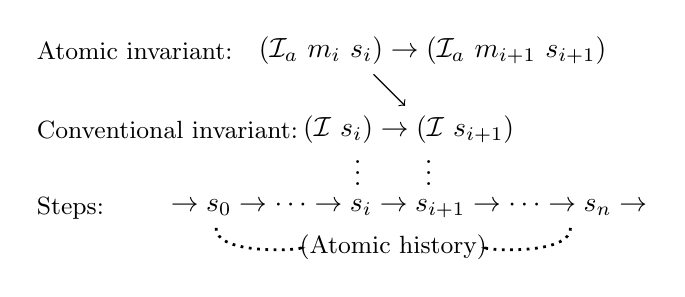
\begin{tikzpicture}
      \node[anchor=west] at (-1.7, 2) {{\small Atomic invariant:}};
      \node[anchor=west] at (1.12, 2) {$(\mathcal{I}_a\ \listof{m_i}\ s_i) \to (\mathcal{I}_a\ \listof{m_{i+1}}\ s_{i+1})$};
      \draw [->] (2.7, 1.7) -- (3.1, 1.3);
      \node[anchor=west] at (-1.7, 1) {{\small Conventional invariant:}};
      \node[anchor=west] at (1.68, 1) {$(\mathcal{I}\ s_i) \to (\mathcal{I}\ s_{i+1})$};
      \node at (2.5, 0.55) {$\vdots$};
      \node at (3.4, 0.55) {$\vdots$};
      \node[anchor=west] at (-1.7, 0) {{\small Steps:}};
      \node[anchor=west] at (0, 0) {$\to s_0 \to \cdots \to s_i \to s_{i+1} \to \cdots \to s_n \to$};
      \node at (2.95, -0.5) {{\small (Atomic history)}};
      \draw [dotted, line width=1pt] (0.7, -0.25) to[out=-90,in=0] (1.7, -0.5);
      \draw [dotted, line width=1pt] (5.2, -0.25) to[out=-90,in=-180] (4.2, -0.5);
    \end{tikzpicture}\\
    \hline
  \end{tabular}
  \caption{Use of atomic invariants in conventional invariant proofs}
  \label{fig-use-atomic-inv}
\end{figure}

\autoref{fig-use-atomic-inv} explains how to use an atomic invariant $\mathcal{I}_a$ while proving a conventional invariant $\mathcal{I}$ in the [TrsAtomic] case.
The point is that we can employ both $(\mathcal{I}\ s_i)$ and $(\mathcal{I}_a\ \listof{m_i}\ s_i)$ to prove $(\mathcal{I}\ s_{i+1})$.
For instance, we may want to have an invariant claiming that the M status uniquely exists, if any, within the system.
(We will indeed use this invariant in our case studies, although the exact statement is a bit more complex.)
The predicate messages defined in \autoref{fig-ex-atomic-invariants} will play a crucial role here, \eg{} the one for \idmsf{8}{rsM} says that $C_1$ and $P$ both have the I status, which means that the state transition by $(r_2: C_2.\textrm{st} \leftarrow M)$ preserves the invariant.

The other three cases ([TrsSilent], [TrsIns], and [TrsOuts]) do not need any further information, since these cases induce just a single step.
We will see more comprehensive uses of predicate messages in our case studies (\autoref{sec-case-study}).

\section{The Hemiola Domain-Specific Language}
\label{sec-hemiola-dsl}

As explained in \autoref{sec-sz-in-hemiola}, on top of serializability it is much easier to design and prove invariants.
That being said, it will be still a large burden if a user has to prove the serializability per-protocol.

In this section, we would like to provide \emph{minimal and abstract conditions} to prove serializability, in order not to prove it for each protocol.
The conditions have been already mentioned with the motivating example in \autoref{sec-example} -- network topology and locking mechanisms, extracted from transient states of practical cache-coherence protocols.

While conventional approaches to verifying cache-coherence protocols deal with transient states directly and induce noninterference lemmas per-state, \hemiola{} provides the serializability guarantee as \emph{the most general form of noninterference, obtained from the conditions that are not coupled with any specific cache-coherence protocols}.

In order to satisfy such conditions for free, \hemiola{} limits protocols primarily by dictating network topologies and locking disciplines and by forcing rules to be defined using \emph{rule templates}.
We will present how the network topologies and the rule templates look like and explain the intuition why using these components implies serializability as well as the actual proof using a technique called \emph{commuting reductions}.

\subsection{The Domain-Specific Language}

\subsubsection{Topology and Network Requirements}
\label{sec-topo-net-reqs}

In order to employ the serializability guarantee in \hemiola{}, the objects in a given system should form a tree topology.
Most cache-coherent memory subsystems follow this topology, where leaf nodes correspond to L1 caches, and the root corresponds to the main memory.
A child and its parent in the tree communicate using the three channels shown in \autoref{sec-example}.
%% \eg{} whenever a child wants to send a request to the parent, it should use the upward-request channel.

\hemiola{} as a Coq library generates the topology and network channels automatically from instances of a simple inductive type.
For example, the following tree definition will generate topology and channels for four L1 caches, two L2 caches, the last-level cache (LLC), and the main memory:
\begin{displaymath}
  t : \textit{tree} \triangleq \small{\textsf{Node [Node [Node [Leaf; Leaf]; Node [Leaf; Leaf]]]}}.
\end{displaymath}

\subsubsection{Locking Mechanism}
\label{sec-locking-mechanism}

We saw in \autoref{sec-example} why fine-grained transient states are required to ensure safe interleavings in cache-coherence protocols.
Revisiting the issue described in \autoref{fig-motive-2}, a child should be able to handle an invalidation request from the parent even if it is in a transient state (SM) and after the response it changes its transient state to IM.
By looking at these transient states carefully, we have discovered that another necessary condition, other than the tree-topology condition, is the locking perspective from the transient states.

\hemiola{} supports a general locking mechanism reflecting this discovery;
instead of looking at the type of a message (\eg{} invalidation), the framework provides \emph{more general} locking, just by looking at whether the message is from the parent or one of its children.
This relaxed locking mechanism is then not coupled with any specific cache-coherence protocols but is still sufficient to prove serializability.

\tikzset{
  uprightedge/.pic = {
    \draw [>->] (0.2, 0.25) -- (0.5, 0.75);
  },
}
\begin{figure}[h]
  \begin{tikzpicture}
    \node at (0, 0) {$C$};
    \pic at (0, 0) {uprightedge};
    \node[label={[label distance=-6pt]right:{\small {\sf rq1}}}] at (0.35, 0.5) {$\bullet$};
    \node at (0.7, 1) {$P_1$};
    \pic at (0.7, 1) {uprightedge};
    \node[label={[label distance=-6pt]left:{\small {\sf rq2}}}] at (1.05, 1.5) {$\bullet$};
    \node at (1.4, 2) {$P_2$};

    \draw [>=stealth,double,->] (1.6, 1.75) -- (1.9, 1.25);
    \node[label={[label distance=-4pt]right:{\small $\overline{\textsf{rqs}}$}}] at (1.75, 1.5) {$\bullet$};

    \node[draw,align=left] at (2.9, 0.4) {$P_1$ sets an uplock\\ when sending {\small $\textsf{rq2}$} to $P_2$};
    \node[draw,align=left] at (4.8, 1.7) {$P_2$ sets a downlock\\ when sending {\small $\overline{\textsf{rqs}}$} to children};
  \end{tikzpicture}
  \caption{Locking mechanism in Hemiola}
  \label{fig-locking}
\end{figure}

In particular, \hemiola{} provides two kinds of locks: \emph{uplocks and downlocks}.
We say an object is uplocked (or downlocked) when it holds an uplock (or downlock), respectively.
\autoref{fig-locking} depicts the locking mechanism in \hemiola{}.
An uplock is set when an object makes an upward request to its parent ($P_1$ in the figure); it is released when the object gets a corresponding response from the parent.
The object cannot make any further upward requests while uplocked, but \emph{it can handle requests from the parent}.
On the contrary, a downlock is set when an object makes a downward request(s) to some of its children ($P_2$ in the figure); similarly it is released when the object gets corresponding response(s) from the child requestee(s).
The object cannot make any further downward requests while downlocked.

Now every cache object defined in \hemiola{} does not need to set transient states to consider all combinations among stable statuses;
instead of it, the framework suggests to maintain the cache status and to set a proper lock.
For example, instead of setting a transient state SM, it is now desirable to maintain its status S and to set an uplock to record it just made the upward request.
(The framework provides even more, actually, by guiding users to employ the \emph{rule templates}, introduced in the next section, that automatically set proper locks.)

Each object defined in \hemiola{} has a semantic \emph{lock state}, a finite map from a lock type (uplock or downlock) to lock information: the original request message, the original requestor index, and requestee indices that are expected to get responses from.
In cache-coherence protocols, each lock corresponds to a miss status holding register (MSHR), a very well-known register used within a cache.
An MSHR is set when a cache miss happens and the miss triggers further requests to obtain a proper status and up-to-date data.
As with \hemiola{} lock holders, MSHRs play a crucial role both in deciding whether to handle certain requests and in storing information needed to handle them properly.

\subsubsection{Rule Templates}
\label{sec-rule-templates}

\newcommand{\rtname}[1]{{\small\sf\bf #1}}

\newcommand{\uled}{\ensuremath{\textsf{UL}}}
\newcommand{\dled}{\ensuremath{\textsf{DL}}}
\newcommand{\ulfree}{\ensuremath{\textsf{UL}_{\times}}}
\newcommand{\dlfree}{\ensuremath{\textsf{DL}_{\times}}}

\newcommand{\setul}{\ensuremath{\textsf{UL}\Uparrow}}
\newcommand{\setdl}{\ensuremath{\textsf{DL}\Uparrow}}
\newcommand{\relul}{\ensuremath{\textsf{UL}\Downarrow}}
\newcommand{\reldl}{\ensuremath{\textsf{DL}\Downarrow}}
\newcommand{\stsilent}{\ensuremath{\textsf{SLT}}}

\newcommand{\ppo}[3]{\ensuremath{\{#1\}#2\lbrack#3\rbrack}}
\newcommand*{\bfrac}[2]{\genfrac{}{}{0pt}{}{#1}{#2}}

\begin{figure}[t]
  \centering
  \begin{subfigure}[b]{0.32\columnwidth}
    \centering
    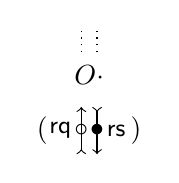
\begin{tikzpicture}
      \draw [dotted] (-0.1, 0.5) -- (-0.1, 0.8);
      \draw [dotted] (0.1, 0.5) -- (0.1, 0.8);
      \node at (0, 0.2) {$\ppo{\bfrac{\ulfree{}}{\dlfree{}}}{O}{\cdot}$};
      \draw [<-<] (-0.1, -0.2) -- (-0.1, -0.8);
      \draw [>->] (0.1, -0.2) -- (0.1, -0.8);
      \node[label={[label distance=-6pt]left:{\small {\sf rq}}}] at (-0.1, -0.5) {$\circ$};
      \node[label={[label distance=-6pt]right:{\small {\sf rs}}}] at (0.1, -0.5) {$\bullet$};
      \node at (0, -0.5) {$(\qquad\quad)$};
    \end{tikzpicture}
    \captionsetup{labelformat=empty}
    \caption{(a) \rtname{immd}}
  \end{subfigure}
  \begin{subfigure}[b]{0.32\columnwidth}
    \centering
    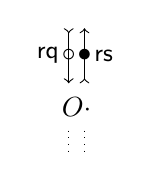
\begin{tikzpicture}
      \draw [<-<] (-0.1, 0.1) -- (-0.1, 0.8);
      \draw [>->] (0.1, 0.1) -- (0.1, 0.8);
      \node at (0, -0.2) {$\ppo{\dlfree{}}{O}{\cdot}$};
      \draw [dotted] (-0.1, -0.5) -- (-0.1, -0.8);
      \draw [dotted] (0.1, -0.5) -- (0.1, -0.8);
      \node[label={[label distance=-6pt]left:{\small {\sf rq}}}] at (-0.1, 0.45) {$\circ$};
      \node[label={[label distance=-6pt]right:{\small {\sf rs}}}] at (0.1, 0.45) {$\bullet$};
    \end{tikzpicture}
    \captionsetup{labelformat=empty}
    \caption{(b) \rtname{immu}}
  \end{subfigure}
  \begin{subfigure}[b]{0.32\columnwidth}
    \centering
    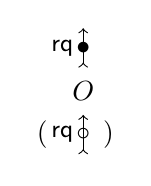
\begin{tikzpicture}
      \draw [>->] (0, 0.3) -- (0, 0.8);
      \node at (0, 0) {$\ppo{\ulfree{}}{O}{\bfrac{\setul{}}{\stsilent{}}}$};
      \draw [<-<] (0, -0.3) -- (0, -0.8);
      \node[label={[label distance=-6pt]left:{\small {\sf rq}}}] at (0, -0.55) {$\circ$};
      \node[label={[label distance=-6pt]left:{\small {\sf rq}}}] at (0, 0.55) {$\bullet$};
      \node at (-0.1, -0.55) {$(\qquad)$};
    \end{tikzpicture}
    \captionsetup{labelformat=empty}
    \caption{(c) \rtname{rquu}}
  \end{subfigure}
  \begin{subfigure}[b]{0.32\columnwidth}
    \centering
    \vspace{5pt}
    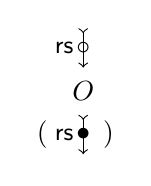
\begin{tikzpicture}
      \draw [<-<] (0, 0.3) -- (0, 0.8);
      \node at (0, 0) {$\ppo{\bfrac{\uled{}}{\dlfree{}}}{O}{\relul{}}$};
      \draw [>->] (0, -0.3) -- (0, -0.8);
      \node[label={[label distance=-6pt]left:{\small {\sf rs}}}] at (0, 0.55) {$\circ$};
      \node[label={[label distance=-6pt]left:{\small {\sf rs}}}] at (0, -0.55) {$\bullet$};
      \node at (-0.1, -0.55) {$(\qquad)$};
    \end{tikzpicture}
    \captionsetup{labelformat=empty}
    \caption{(d) \rtname{rsdd}}
  \end{subfigure}
  \begin{subfigure}[b]{0.32\columnwidth}
    \centering
    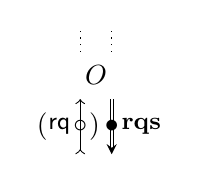
\begin{tikzpicture}
      \draw [dotted] (-0.2, 0.5) -- (-0.2, 0.8);
      \draw [dotted] (0.2, 0.5) -- (0.2, 0.8);
      \node at (0, 0.2) {$\ppo{\dlfree{}}{O}{\bfrac{\setdl{}}{\stsilent{}}}$};
      \draw [<-<] (-0.2, -0.1) -- (-0.2, -0.8);
      \draw [>=stealth,double,->] (0.2, -0.1) -- (0.2, -0.8);
      \node[label={[label distance=-6pt]left:{\small {\sf rq}}}] at (-0.2, -0.45) {$\circ$};
      \node[label={[label distance=-6pt]right:{\small {\sf {\bf rqs}}}}] at (0.2, -0.45) {$\bullet$};
      \node at (-0.35, -0.45) {$(\enspace\quad)$};
    \end{tikzpicture}
    \captionsetup{labelformat=empty}
    \caption{(e) \rtname{rqud}}
  \end{subfigure}
  \begin{subfigure}[b]{0.32\columnwidth}
    \centering
    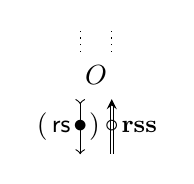
\begin{tikzpicture}
      \draw [dotted] (-0.2, 0.5) -- (-0.2, 0.8);
      \draw [dotted] (0.2, 0.5) -- (0.2, 0.8);
      \node at (0, 0.2) {$\ppo{\dled{}}{O}{\reldl{}}$};
      \draw [>->] (-0.2, -0.1) -- (-0.2, -0.8);
      \draw [>=stealth,double,<-] (0.2, -0.1) -- (0.2, -0.8);
      \node[label={[label distance=-6pt]left:{\small {\sf rs}}}] at (-0.2, -0.45) {$\bullet$};
      \node[label={[label distance=-6pt]right:{\small {\sf {\bf rss}}}}] at (0.2, -0.45) {$\circ$};
      \node at (-0.35, -0.45) {$(\enspace\quad)$};
    \end{tikzpicture}
    \captionsetup{labelformat=empty}
    \caption{(f) \rtname{rsud}}
  \end{subfigure}
  \begin{subfigure}[b]{0.32\columnwidth}
    \centering
    \vspace{5pt}
    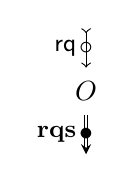
\begin{tikzpicture}
      \draw [<-<] (0, 0.3) -- (0, 0.8);
      \node at (0, 0) {$\ppo{\dlfree{}}{O}{\bfrac{\setdl{}}{\stsilent{}}}$};
      \draw [>=stealth,double,->] (0, -0.3) -- (0, -0.8);
      \node[label={[label distance=-6pt]left:{\small {\sf rq}}}] at (0, 0.55) {$\circ$};
      \node[label={[label distance=-6pt]left:{\small {\sf {\bf rqs}}}}] at (0, -0.55) {$\bullet$};
    \end{tikzpicture}
    \captionsetup{labelformat=empty}
    \caption{(g) \rtname{rqdd}}
  \end{subfigure}
  \begin{subfigure}[b]{0.32\columnwidth}
    \centering
    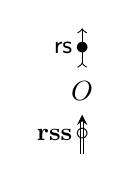
\begin{tikzpicture}
      \draw [>->] (0, 0.3) -- (0, 0.8);
      \node at (0, 0) {$\ppo{\dled{}}{O}{\reldl{}}$};
      \draw [>=stealth,double,<-] (0, -0.3) -- (0, -0.8);
      \node[label={[label distance=-6pt]left:{\small {\sf rs}}}] at (0, 0.55) {$\bullet$};
      \node[label={[label distance=-6pt]left:{\small {\sf {\bf rss}}}}] at (0, -0.55) {$\circ$};
    \end{tikzpicture}
    \captionsetup{labelformat=empty}
    \caption{(h) \rtname{rsuu}}
  \end{subfigure}
  \begin{subfigure}[b]{0.32\columnwidth}
    \centering
    \begin{tikzpicture}
      \draw [<-<] (0, 0.3) -- (0, 0.8);
      \node at (0, 0) {$\ppo{\bfrac{\uled{}}{\dlfree{}}}{O}{\bfrac{\relul{}}{\setdl{}}}$};
      \draw [>=stealth,double,->] (0, -0.3) -- (0, -0.8);
      \node[label={[label distance=-6pt]left:{\small {\sf rs}}}] at (0, 0.55) {$\circ$};
      \node[label={[label distance=-6pt]left:{\small {\sf {\bf rqs}}}}] at (0, -0.55) {$\bullet$};
    \end{tikzpicture}
    \captionsetup{labelformat=empty}
    \caption{(i) \rtname{rsrq}}
  \end{subfigure}
  \caption{Rule templates in \hemiola{}}
  \label{fig-rule-templates}
\end{figure}

In order to establish the topology/network requirements and the locking mechanism automatically, \hemiola{} provides rule templates that make state transitions within the conditions.
\autoref{fig-rule-templates} presents the nine rule templates supported in \hemiola{}.
Each diagram has the form $\ppo{P}{O}{Q}$ and arrows with the circles ($\circ$ and $\bullet$) and the labels representing requests (\msgsfsm{rq(s)}) and responses (\msgsfsm{rs(s)}).
It means that the rule template is for an object $O$, requires input messages ($\circ$) with the the message types determined by the label, has a precondition $P$, performs a state transition $Q$, and generates output messages ($\bullet$).

$\uled$, $\dled$, $\ulfree$, and $\dlfree$ in a precondition indicate that the object should be uplocked, downlocked, uplock-free, and downlock-free, respectively.
$\setul$, $\setdl$, $\relul$, and $\reldl$ in a state transition indicate setting an uplock, setting a downlock, releasing an uplock, and releasing a downlock, respectively.
$\stsilent{}$ annotates that the rule template forbids any state modification beside locking.
Looking at the rules one-by-one:
\begin{enumerate}[label=(\alph*),leftmargin=*]
\item \rtname{immd} responds immediately to an upward request. It can make a local state transition without any input/output messages as well (input/output messages marked with parentheses in \autoref{fig-rule-templates}).
\item \rtname{immu} responds immediately to a downward request.
\item \rtname{rquu} (possibly) takes an upward request and requests to its parent.
\item \rtname{rsdd} takes a downward response and (possibly) responds to the original child requestor.
\item \rtname{rqud} (possibly) takes an upward request and requests to some of its children.
\item \rtname{rsud} takes upward responses and (possibly) responds to the original child requestor.
\item \rtname{rqdd} takes a downward request and requests to some of its children.
\item \rtname{rsuu} takes upward responses and responds to its parent.
\item \rtname{rsrq} takes a downward response and requests to some of its children.
\end{enumerate}

The rule templates are carefully designed to perform any practical transactions \emph{safely} with serializable behavior.
Considering an extreme case, in a cache-coherence protocol, if an L1 cache wants to obtain a write permission, all the other caches should be invalidated (changing each cache status to Invalid).
In order to perform such a transaction, it must be able to traverse all the other caches.
This transaction kind is one of the longest-running in cache-coherence protocols, and the rule templates are designed with proper locking ($\uled$ and $\dled$) and a state-change condition ($\stsilent$), not to create any incoherence while such a long transaction is interleaved with other transactions.

\newcommand{\rdcircfl}[2]{\rdcircf{#1}{#2}}
\newcommand{\rdcircflsm}[2]{\rdcircf{#1}{\footnotesize #2}}
\newcommand{\blcircfl}[2]{\blcircf{#1}{#2}}
\newcommand{\blcircflsm}[2]{\blcircf{#1}{\footnotesize #2}}

\begin{figure*}[t]
  \begin{subfigure}[b]{0.3\textwidth}
    \centering
    \begin{tabular}{c}
      \begin{tikzpicture}
        \pic at (0, 0) {skeleton-pcce1={$P$}{$C_1$}{$C_2$}};
        % C_1 external
        \pic at (0, 0) {skeleton-midx-e1};
        \node[label={[label distance=-6pt,myred]left:{\small {\sf rqWr}}},color=myred] at (-1.6, -2.05) {$\bullet$};
        \node[label={[label distance=-6pt,myred]right:{\small {\sf rsWr}}},color=myred] at (-1.4, -2.05) {$\bullet$};
        % Between P and C_1
        \pic at (0, 0) {skeleton-midx-pc1};
        \node[label={[label distance=-6pt,myred]left:{\small {\sf rqM}}},color=myred] at (-1, -0.7) {$\bullet$};
        \node[label={[label distance=-9pt,myred]below right:{\small {\sf rsM}}},color=myred] at (-0.6, -0.7) {$\bullet$};
        % Between P and C_2
        \pic at (0, 0) {skeleton-midx-pc2};
        \node[label={[label distance=-9pt,myred]below left:{\small {\sf rsI}}},color=myred] at (0.8, -0.7) {$\bullet$};
        \node[label={[label distance=-6pt,myred]right:{\small {\sf rqI}}},color=myred] at (1, -0.7) {$\bullet$};

        % Curves
        \draw [->,color=myred] (-2.1, -1.8) to[out=90,in=-90] node[left] {\rdcircflsm{1}{rquu}} (-1.6, -0.9);
        \draw [->,color=myred] (-1.6, -0.5) to[out=70,in=110,distance=1.4cm] node[left=15pt] {\rdcircflsm{3}{rqud}} (1.4, -0.4);
        \draw [->,color=myred] (1.5, -0.9) to[out=-50,in=-50,distance=1.5cm] node[below] {\rdcircflsm{4}{immu}} (0.5, -1.1);
        \draw [->,color=myred] (0.4, -0.8) to[out=135,in=45,distance=0.6cm] (-0.3, -0.7);
        \draw [densely dashed,color=myred,line width=0.3pt] (0, -0.35) to[out=90,in=-170] (1.3, 0.35);
        \node at (1.7, 0.3) {\rdcircflsm{5}{rsud}};
        \draw [->,color=myred] (-0.6, -1.1) to[out=225,in=90] node[below right] {\rdcircflsm{7}{rsdd}} (-1.1, -1.8);
      \end{tikzpicture}\\
      %% {\bf (a) The {\color{myred} red} transaction }\\
      \begin{tikzpicture}
        \pic at (0, 0) {skeleton-pcce2={$P$}{$C_1$}{$C_2$}};
        % C_2 external
        \pic at (0, 0) {skeleton-midx-e2};
        \node[label={[label distance=-6pt,myblue]right:{\small {\sf rsWr}}},color=myblue] at (1.6, -2.05) {$\bullet$};
        \node[label={[label distance=-6pt,myblue]left:{\small {\sf rqWr}}},color=myblue] at (1.4, -2.05) {$\bullet$};
        % Between P and C_1
        \pic at (0, 0) {skeleton-midx-pc1};
        \node[label={[label distance=-9pt,myblue]above left:{\small {\sf rsI}}},color=myblue] at (-0.8, -0.7) {$\bullet$};
        \node[label={[label distance=-10pt,myblue]below right:{\small {\sf rqI}}},color=myblue] at (-0.6, -0.7) {$\bullet$};
        % Between P and C_2
        \pic at (0, 0) {skeleton-midx-pc2};
        \node[label={[label distance=-6pt,myblue]right:{\small {\sf rsM}}},color=myblue] at (1, -0.7) {$\bullet$};
        \node[label={[label distance=-10pt,myblue]below left:{\small {\sf rqM}}},color=myblue] at (0.6, -0.7) {$\bullet$};

        % Curves
        \draw [->,color=myblue] (1.1, -1.8) to[out=90,in=-45] node[below left=-3pt] {\blcircflsm{2}{rquu}} (0.6, -1.1);
        \draw [->,color=myblue] (0.3, -0.7) to[out=135,in=45,distance=0.5cm] (-0.3, -0.7);
        \draw [densely dashed,color=myblue,line width=0.3pt] (0, -0.35) to[out=90,in=-170] (1.3, 0.35);
        \node at (1.7, 0.3) {\blcircflsm{6}{rqud}};
        \draw [->,color=myblue] (-0.5, -1.1) to[out=-135,in=-135,distance=1.8cm] node[below] {\blcircflsm{8}{immu}} (-1.3, -0.7);
        \draw [->,color=myblue] (-1.1, -0.3) to[out=60,in=120,distance=1.3cm] node[left=17pt] {\blcircflsm{9}{rsud}} (1.4, -0.5);
        \draw [->,color=myblue]  (1.6, -0.95) to[out=-90,in=90] node[above right=-2pt] {\blcircflsm{10}{rsdd}} (2.1, -1.8);
      \end{tikzpicture}
    \end{tabular}
    \caption{The two transactions}
    \label{fig-ex-sz-trs}
  \end{subfigure}
  \begin{subfigure}[b]{0.5\textwidth}
    \renewcommand{\arraystretch}{1.2}
    \setlength\tabcolsep{2.5pt}
    \small\centering
    \begin{tabular}{c}
      \multicolumn{1}{l}{
        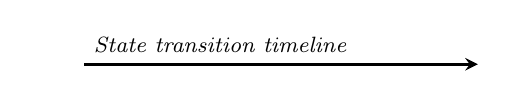
\begin{tikzpicture}
          \node at (-0.6, 0) {};
          \node[anchor=west] at (0, 0.25) {{\footnotesize\it State transition timeline}};
          \draw [>=stealth,->,line width=1pt] (0, 0) to (5, 0);
        \end{tikzpicture}}\\
      \begin{tabular}{c|ccccccccccc}
        \hline
        $C_1$ & & \rdcircf{1} & & & & & & \rdcircf{7} & \blcircf{8} & & \\
        \hline
        $P$ & & & & \rdcircf{3} & & \rdcircf{5} & \blcircf{6} & & & \blcircf{9} & \\
        \hline
        $C_2$ & & & \blcircf{2} & & \rdcircf{4} & & & & & & \blcircf{10} \\
        \hline
      \end{tabular}\\
      \vspace{-10pt}\\
      $\downarrow$ (\blcircf{6} and \rdcircf{7} commute)\\
      \vspace{-10pt}\\
      \begin{tabular}{c|ccccccccccc}
        \hline
        $C_1$ & & \rdcircf{1} & & & & & \rdcircf{7} & & \blcircf{8} & & \\
        \hline
        $P$ & & & & \rdcircf{3} & & \rdcircf{5} & & \blcircf{6} & & \blcircf{9} & \\
        \hline
        $C_2$ & & & \blcircf{2} & & \rdcircf{4} & & & & & & \blcircf{10} \\
        \hline
      \end{tabular}\\
      \vspace{-10pt}\\
      $\downarrow$ ($[\rdcircf{3}; \rdcircf{4}; \rdcircf{5}; \rdcircf{7}]$ and $[\blcircf{2}]$ commute)\\
      \vspace{-10pt}\\
      \begin{tabular}{c|ccccccccccc}
        \hline
        $C_1$ & & \rdcircf{1} & & & & \rdcircf{7} & & & \blcircf{8} & & \\
        \hline
        $P$ & & & \rdcircf{3} & & \rdcircf{5} & & & \blcircf{6} & & \blcircf{9} & \\
        \hline
        $C_2$ & & & & \rdcircf{4} & & & \blcircf{2} & & & & \blcircf{10} \\
        \hline
      \end{tabular}
    \end{tabular}
    \renewcommand{\arraystretch}{1.0}
    \caption{Serialization of an interleaved history by reductions}
    \label{fig-ex-sz-state-trs}
  \end{subfigure}
  \begin{subfigure}[b]{0.18\textwidth}
    \centering
    \begin{tabular}{c}
      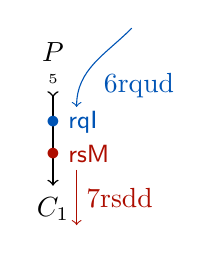
\begin{tikzpicture}
        \node at (0, 0.5) {$P$};
        \node at (0, 0.15) {\tiny $5$};
        \draw [line width=0.2mm, >->] (0, 0) -- (0, -1.2);
        \node[label={[label distance=-4pt,myblue]right:{\small {\sf rqI}}},color=myblue] at (0, -0.4) {$\bullet$};
        \node[label={[label distance=-4pt,myred]right:{\small {\sf rsM}}},color=myred] at (0, -0.8) {$\bullet$};
        \node at (0, -1.5) {$C_1$};

        % Curves
        \draw [->,color=myblue] (1, 0.8) to[out=-135,in=90] node[below right] {\blcircflsm{6}{rqud}} (0.3, -0.2);
        \draw [->,color=myred] (0.3, -1.0) to[out=-90,in=90] node[right] {\rdcircflsm{7}{rsdd}} (0.3, -1.7);
      \end{tikzpicture}\\
      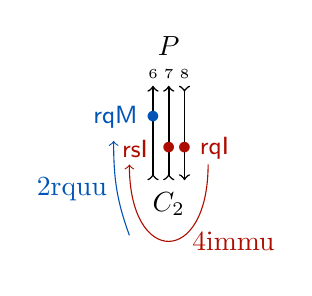
\begin{tikzpicture}
        \node at (0, 0.5) {$P$};
        \node at (-0.2, 0.15) {\tiny $6$};
        \node at (0, 0.15) {\tiny $7$};
        \node at (0.2, 0.15) {\tiny $8$};
        \draw [line width=0.2mm, <-<] (-0.2, 0) -- (-0.2, -1.2);
        \draw [line width=0.2mm, <-<] (0, 0) -- (0, -1.2);
        \draw [line width=0.2mm, >->] (0.2, 0) -- (0.2, -1.2);
        \node[label={[label distance=-4pt,myblue]left:{\small {\sf rqM}}},color=myblue] at (-0.2, -0.4) {$\bullet$};
        \node[label={[label distance=-2pt,myred]left:{\small {\sf rsI}}},color=myred] at (0, -0.8) {$\bullet$};
        \node[label={[label distance=-4pt,myred]right:{\small {\sf rqI}}},color=myred] at (0.2, -0.8) {$\bullet$};
        \node at (0, -1.5) {$C_2$};

        % Curves
        \draw [->,color=myblue] (-0.5, -1.9) to[out=110,in=-90] node[left] {\blcircflsm{2}{rquu}} (-0.7, -0.7);
        \draw [->,color=myred] (0.5, -1.0) to[out=-90,in=-90,distance=1.3cm] node[right=5pt] {\rdcircflsm{4}{immu}} (-0.5, -1.0);
      \end{tikzpicture}\\
    \end{tabular}
    \caption{Reduction cases}
    \label{fig-ex-sz-comm}
  \end{subfigure}
  \caption{Interleaving transactions and their serialization by commuting rule-template-based state transitions}
  \label{fig-ex-sz}
\end{figure*}

Each rule in the templates sets/releases a lock properly, depending on which messages the rule takes and generates.
While the locking mechanism was explained in \autoref{sec-locking-mechanism}, we still see a number of interesting cases that are worth analyzing again in terms of correctness and liveness:
\begin{itemize}[leftmargin=*]
\item \rtname{\{immd, rquu, rqud\}} show that a transaction may start without any input messages as a trigger, which still matches the definition of externally atomic histories in \autoref{fig-trs-semantics}. On the other hand, \rtname{\{immd, rsdd, rsud\}} show that a transaction may not generate output messages.
\item \rtname{\{immu, rqdd\}} show that an object can handle a request from the parent even when uplocked. These rules do not have a precondition that the object should be uplock-free. Note again that this relaxation is to avoid a deadlock.
\item \rtname{rsdd} says that in order to handle a response from the parent, the object should be downlock-free. This precondition is indeed required to ensure serializability.
\item \rtname{rsrq} forces the order of a traversal, saying that the traversal for the outer objects must be done before traversing the inner objects. The forced order is important to avoid a deadlock. For example, if the object makes requests to its parent and children at the same time and sets both an uplock and a downlock, a deadlock may occur.
\end{itemize}

%% \todo{How to convince that the Hemiola locks are not overused?}
%% \todo{Clarify this paragraph more, or consider removing it.}
%% A reader may wonder if there is a rule template that \emph{overuses} locks, \ie{} one with an unnecessary check that a certain lock is free.
%% We argue that the rule templates are also carefully designed not to have such cases; quite the contrary, we found another implementation~\cite{Zhang:2019,thesis:Zhang:2019}, a cache-coherence protocol written in the Bluespec HDL (hardware description language)~\cite{bluespec}, that overused a lock in a specific situation, although their current cache-coherence protocol does not have any cases that may benefit from this relaxation.
%% Looking at the rule template \rtname{rquu}, we see that the downlock-free ($\dlfree$) condition is \emph{not} required to make an upward request to the parent.
%% This choice is safe since the upward request may introduce state changes outside the object until it takes a corresponding downward response (see \rtname{rsdd}, which checks downlock-freedom when taking the response).
%% Their implementation, however, blocks the upward request when a downlock is set, even if it is (proven to be) safe to relax it.
%% We believe this case provides evidence that a carefully predesigned locking mechanism helps with efficient locking placement.

\subsection{Serializability Guarantee by the \hemiola{} DSL}

We now present the intuition and the sketch of the serializability proof for the protocols satisfying the topology/network condition (\autoref{sec-topo-net-reqs}) and the locking mechanism (\autoref{sec-locking-mechanism}).
In proving serializability we use a well-established technique called commuting reductions~\cite{reduction}.
This reduction technique has been used before to prove correctness of concurrent software~\cite{Chajed:2018} and distributed systems~\cite{Hawblitzel:2015,Hawblitzel:2017}, but no past work has tried to discover new serializability conditions that can fit for cache-coherence protocols and to prove it using reductions.

We say that two adjacent state transitions \emph{commute} if the state transitions with the opposite order reach to the same state:
$\semstep{S}{s_0}{l_0}{s_1} \to \semstep{S}{s_1}{l_1}{s_2} \to \exists s_1'.\; \semstep{S}{s_0}{l_1}{s_1'} \to \semstep{S}{s_1'}{l_0}{s_2}$.
We can naturally lift the notion for histories to argue whether two histories commute or not.
Our high-level intuition for the serializability proof is that for a given interleaved history we can perform a finite number of reductions to get a sequential history that reaches the same state.
More specifically, we will try to \emph{merge} two separated atomic-history fragments by performing reductions.
%% If it is enforced that no other atomic fragments are split during this merge, we can eventually get the sequential history by performing a finite number of merges.

We elaborate more on this intuition with \autoref{fig-ex-sz}: two interleaving transactions started from $C_1$ and $C_2$, respectively, both pursuing the M status from the simple MSI protocol presented in \autoref{sec-example}.
The two transactions are presented in \autoref{fig-ex-sz-trs} by {\color{myred} red} and {\color{myblue} blue} colors.
We use an arrow ({\color{myred} $\to$}) and a label (\rdcircfl{1}{rquu}) to denote a state transition by a rule defined with a certain rule template, \eg{} \rdcircfl{1}{rquu} is a rule in $C_1$ using the ``rquu'' rule template, that takes an input message \idmsf{1}{rqWr} and outputs \idmsf{3}{rqM}.

%% \begin{itemize}[leftmargin=*]
%% \item \rdcircfl{1}{rquu} (or \blcircfl{2}{rquu}): forward \msgsfsm{rqM} to $P$ since $C_1$ (or $C_2$) does not have the M status.
%% \item \rdcircfl{3}{rqud} (or \blcircfl{6}{rqud}): $P$ makes an invalidation request to the other child.
%% \item \rdcircfl{4}{immu} (or \blcircfl{8}{immu}): change the status to I and respond with \msgsfsm{rsI} immediately.
%% \item \rdcircfl{5}{rsud} (or \blcircfl{9}{rsud}): the invalidation has finished so $P$ responds with \msgsfsm{rsM} to the original requestor.
%% \item \rdcircfl{7}{rsdd} (or \blcircfl{10}{rsdd}): $C_1$ (or $C_2$) takes the response and updates its status to M.
%% \end{itemize}

\autoref{fig-ex-sz-state-trs} shows how reductions apply to the original interleaved history (top) to make it sequential (bottom).
In order to merge $[\rdcircf{3}; \rdcircf{4}; \rdcircf{5}]$ and $[\rdcircf{7}]$, we should perform a reduction either between $[\rdcircf{3}; \rdcircf{4}; \rdcircf{5}]$ and $[\blcircf{6}]$ or between $[\blcircf{6}]$ and $[\rdcircf{7}]$.
From the perspective of this kind of merge, we will say that $[\blcircf{6}]$ is \emph{pushed} to the left (or right) when it commutes with $[\rdcircf{3}; \rdcircf{4}; \rdcircf{5}]$ (or $[\rdcircf{7}]$), respectively.

Two state transitions trivially commute if 1) the object state transitions happen in the different objects and 2) input/output channels used for the transitions are all orthogonal to each others.
If either of the conditions does not hold, we may need to analyze more whether the transitions commute or not.
In this merge case, $[\blcircf{6}]$ can be pushed to the right (\ie{} \blcircf{6} and \rdcircf{7} commute).
The object state transitions are straightforward to deal with, since they are orthogonal ($P$ for \blcircf{6} and $C_1$ for \rdcircf{7}).
It is nontrivial to deal with the used channels, however, since the output of \blcircf{6} (\blmsgsm{rqI}) and the input of \rdcircf{7} (\rdmsgsm{rsM}) share the same channel $5$.
\autoref{fig-ex-sz-comm} (above) depicts this case; we see \blcircf{6} and \rdcircf{7} still commute, since \rdcircfl{7}{rsdd} should take a response (\rdmsgsm{rsM}) while \blcircfl{6}{rqud} outputs a request.
It indicates that \blcircf{6} and \rdcircf{7} are involved with different messages in the same channel, thus not affecting the commutativity.
We obtain a new (less-interleaved) history after the reduction, shown in the middle.

Now we should merge $[\rdcircf{1}]$ and $[\rdcircf{3}; \rdcircf{4}; \rdcircf{5}; \rdcircf{7}]$; in this case, \blcircf{2} can be pushed to the right.
While this reduction is trivial in the sense of orthogonal objects and channels, the only nontrivial case is between \blcircf{2} and \rdcircf{4}, where the both rules are executed in $C_2$.
These state transitions still commute, as shown in \autoref{fig-ex-sz-comm} (below), since \blcircf{2} cannot make any object state transition, according to the definition of the ``rquu'' rule template.

How can we argue that atomic-history fragments are always mergeable?
As seen in the two cases in \autoref{fig-ex-sz-state-trs}, the reason for the mergeability comes only from what have been specified by the rule templates.
It is required to consider all possible reduction cases among the rule templates to prove the serializability.

The biggest contribution of the \hemiola{} framework includes precise formalization of the intuitions -- merging atomic fragments, commutativity among the rule templates, left/right pushes, etc. -- and the serializability proof with the topology/network and rule conditions.
The highest-level theorem simply claims that the use of good topology and the rule templates automatically guarantees serializability:
\newcommand{\ontree}[2]{\ensuremath{\mathsf{OnTree}\ #1\ #2}}
\newcommand{\goodrules}[2]{\ensuremath{\mathsf{GoodRules}\ #1\ #2}}
\begin{theorem}[\hemiola{}'s serializability guarantee]
  \begin{displaymath}
    \forall S, t.\; \ontree{S}{t} \land \goodrules{S}{t} \to \hsrz{S},
  \end{displaymath}
  where $(\ontree{S}{t})$ requires that the system $S$ is well-defined on the topology/network $t$, and $(\goodrules{S}{t})$ requires that each rule in $S$ conforms to one of the rule templates.
  \label{thm-sz-guarantee}
\end{theorem}
While we only provided the intuition why this theorem holds, interested readers are referred to \autoref{sec-appx-sz-guarantee}, which presents the required formalization and the proof of this theorem.
Also, the full mechanized Coq proof is in the supplementary material.

\section{Case Studies: Hierarchical MSI and MESI Protocols}
\label{sec-case-study}

In this section we specify, implement, and formally prove the correctness of hierarchical MSI and MESI protocols as case studies.
They use directories to keep track of child statuses and use noninclusive caches that do not require the parent cache to contain all lines existing in children.
We will see how \hemiola{} helps implement and prove these protocols, by taking full advantage of \autoref{thm-sz-guarantee}.

\subsection{Design Principles}
We start by summarizing the design principles we applied to both case studies.

\subsubsection{Topology as a parameter}
\label{sec-topo-param}
Each design is parameterized by a tree $t$ that decides the topology of the memory subsystem.
In other words, whenever we instantiate the tree parameter, we get a cache-coherence design and its correctness proof for free.
(Contrast with much work on model-checking cache-coherence protocols, where a new analysis must be run for each tree shape.)

There are three different kinds of caches in this topology-parameterized protocol.
First of all, there are L1 caches (denoted as $L_1$) that correspond to leaf nodes in the tree.
Symmetrically, each uses the same set of rules.
The second kind is the last-level cache (LLC), which is the only one attached to the main memory, the root of the tree\footnote{It is possible to design multiple LLCs attached to the main memory in \hemiola{}, but our case studies follow standard practice in sticking to a single LLC.}.
All the other caches between the L1 caches and the LLC are called intermediate caches (denoted as $L_i$), and they share a common set of rules as well.

\subsubsection{Directory-based coherence}

The protocol uses a well-known directory structure~\cite{Tang:1976} to ensure coherence.
In our designs, each node with children has its own directory structure to track their statuses.
The directory holds sound information about the status of each child \emph{subtree}.
For example, for a certain cache line, if an L1 cache $L_1$ has M status for the line, then all the ancestors (including the main memory) of $L_1$ have the directory status M pointing to the child subtree that contains $L_1$.

\subsubsection{Voluntary evictions}

The protocol allows voluntary evictions, \ie{} there are rules in each cache that can be executed even without being triggered by input messages, to evict a cache line.
This design itself is certainly not realistic, but it always has more behaviors than any design with specific eviction policies, thus in terms of correctness a refinement to a specific design is trivial.

\subsubsection{Noninclusiveness}
\label{sec-noninclusive}

The protocol uses the noninclusive-cache inclusive-directory (NCID)~\cite{Zhao:2010} structure to optimize the cache space.
In terms of protocol design, unlike conventional inclusive caches, the parent cache does not have to contain all the line values that children have, and back invalidations are not required to evict a line.
In inclusive caches, in order to maintain the inclusion policy, it is required to invalidate each cache line of a child recursively before evicting the parent's line, which adds overhead.
On the other hand, noninclusive caches do not need such a process.

Measuring performance among various cache-inclusion policies is beyond the scope of this work.
That said, we choose noninclusive caches as our case studies to demonstrate that \hemiola{} is general enough to design and prove various cache-coherence protocols, where specifically the noninclusive caches are the ones that most previous work had difficulty dealing with properly (see \autoref{sec-discussion} for more-detailed discussion).

\subsubsection{Design and proof per-line}
\label{sec-design-line}

The protocol is defined just for a single cache line first, then naturally extended to all cache lines using a protocol compiler that will be introduced in \autoref{sec-synthesis}.
This approach is reasonable in terms of correctness, since a transaction does not affect coherence for lines other than its own.
Consider the ``duplicated'' protocol first, where each cache line, its status, a directory entry, communication channels, and a lock holder are all duplicated per-line.
It is infeasible to extend the protocol literally in this way, since we cannot require physically distinct channels and lock holders for all cache lines.
The protocol compiler restricts the resources (\eg{} channels, lock holders, etc.) to make the implementation hardware-synthesizable.
Note that in this sense the duplicated protocol can be regarded as the most general multiline design, whose behaviors can cover all the behaviors of compiled implementations (see \autoref{sec-compiler} for details).

\subsection{The MSI Protocol}
\label{sec-msi-protocol}

\newcommand{\mesi}{\ensuremath{\textsf{MESI}}}
\newcommand{\msi}{\ensuremath{\textsf{MSI}}}
\newcommand{\stM}{\ensuremath{\textsf{M}}}
\newcommand{\stE}{\ensuremath{\textsf{E}}}
\newcommand{\stS}{\ensuremath{\textsf{S}}}
\newcommand{\stI}{\ensuremath{\textsf{I}}}
\newcommand{\dir}[2]{\ensuremath{#1_{\tuple{#2}}}}

The MSI protocol is known as a base cache-coherence protocol that can be optimized to more sophisticated protocols like MESI, MOSI, etc.
Even though it is a base protocol, there are a lot of nontrivial cases that require deep understanding of the protocol itself and the nature of distributed protocols, especially in hierarchical protocols.
In this section we design a hierarchical, directory-based MSI protocol with design/verification tools supported by \hemiola{}.
As explained in \autoref{sec-design-line}, the description and the correctness proof will be for a single cache line for now.

\subsubsection{Protocol description}

\paragraph{Cache states.}
A cache state has the form $O(\textsf{st}, \textsf{v}, \textsf{dir}, \textsf{owned})$, consisting of a status, a value, a directory, and a Boolean called an \emph{ownership bit}.
A status is either \stM{}, \stS{}, or \stI{}.
A directory contains a status of its children called a \emph{directory status} and a list of child-cache indices that have the directory status.
We will denote the directory like $\dir{\stS{}}{1, 2}$, saying that the directory status is \stS{} and child subtrees with indices $1$ and $2$ may contain caches with \stS{} status.

The ownership bit is to determine whether the cache is responsible for writing the value back to the parent when invalidated.
When a cache has the \stM{} status, the ownership bit is always true.
However, when the cache has \stS{}, the ownership bit can be either true or false.
Note that $L_1$ does not have a directory since it has no children.
It also does not have an ownership bit, since it does not have a case where it has \stS{} status but is responsible for writing the value back.

\tikzset{
  pcc1/.pic = {
    \node at (0, 0) {$P(\stI{}, \cdot, \dir{\stM{}}{1}, \bot)$};
    \node at (-1.1, -1.1) {$C_1(\stM{}, v)$};
    \node at (1.1, -1.1) {$C_2(\stI{}, \cdot)$};
    % to the parent of P
    \node at (0, 1) {$\vdots$};
    \draw [>->] (-0.2, 0.3) -- (-0.2, 0.6);
    \draw [>->] (0, 0.3) -- (0, 0.6);
    \draw [<-<] (0.2, 0.3) -- (0.2, 0.6);
    % between P and C_1
    \draw [<-<] (-0.6, -0.3) -- (-1, -0.8);
    \draw [<-<] (-0.4, -0.3) -- (-0.8, -0.8);
    \draw [>->] (-0.2, -0.3) -- (-0.6, -0.8);
    % between P and C_2
    \draw [<-<] (0.6, -0.3) -- (1, -0.8);
    \draw [<-<] (0.4, -0.3) -- (0.8, -0.8);
    \draw [>->] (0.2, -0.3) -- (0.6, -0.8);
    % message
    \node[label={[label distance=-6pt]right:{\small {\sf rqS}}}] at (0.8, -0.55) {$\bullet$};
  },
  pcc2/.pic = {
    \node at (0, 0) {$P(\stS{}, v, \dir{\stS{}}{1,2}, \top)$};
    \node at (-1.1, -1.1) {$C_1(\stS{}, v)$};
    \node at (1.1, -1.1) {$C_2(\stI{}, \cdot)$};
    % to the parent of P
    \node at (0, 1) {$\vdots$};
    \draw [>->] (-0.2, 0.3) -- (-0.2, 0.6);
    \draw [>->] (0, 0.3) -- (0, 0.6);
    \draw [<-<] (0.2, 0.3) -- (0.2, 0.6);
    % between P and C_1
    \draw [<-<] (-0.6, -0.3) -- (-1, -0.8);
    \draw [<-<] (-0.4, -0.3) -- (-0.8, -0.8);
    \draw [>->] (-0.2, -0.3) -- (-0.6, -0.8);
    % between P and C_2
    \draw [<-<] (0.6, -0.3) -- (1, -0.8);
    \draw [<-<] (0.4, -0.3) -- (0.8, -0.8);
    \draw [>->] (0.2, -0.3) -- (0.6, -0.8);
    % message
    \node[label={[shift={(0.3,-0.2)}]left:{\small {\sf rsS}$(v)$}}] at (0.4, -0.55) {$\bullet$};
  }
}
\begin{figure}[h]
  \centering
  \frame{
    \begin{tikzpicture}
      \pic at (-2.3, 0) {pcc1};
      \node at (0, 0) {$\longrightarrow^{\ast}$};
      \pic at (2.3, 0) {pcc2};
    \end{tikzpicture}
  }
  \caption{An ownership bit set in a shared-state cache}
  \label{fig-ownership-bit}
\end{figure}

\autoref{fig-ownership-bit} presents an example of a shared-state cache having its ownership bit set in a hierarchical memory subsystem.
It could happen when an L1 cache $C_2$ wants to get \stS{} while another L1 cache $C_1$ has \stM{}.
In this case, the value is pulled from $C_1$, and the parent $P$ gets the data as well, entering a shared state with ownership bit set.
Here the bit says that the shared value might be dirty, so it should be written back.
The ownership bit intuitively constrains which caches can have valid status.
In the figure, all the other caches outside $P$, after pulling a value from $C_1$, are in the invalid status, since previously $C_1$ had the dirty value with \stM{}.
We will see how this intuition is used for the correctness proof soon in \autoref{sec-msi-proof}.

\paragraph{Protocol description with rule templates.}

We present a number of rule descriptions in the MSI protocol that employ the rule templates provided in \hemiola{}.
Each rule template is defined in Coq, taking in several parameters and generating a rule.
We exploited Coq's notation mechanism to have a compact definition for each rule template.

\begin{figure}[h]
  \centering
\begin{lstlisting}
Definition l1GetSRqUpUp: Rule :=
  rule.rquu
  :accepts rqS
  :from cidx
  :me oidx
  :requires (fun ost _ => ost#[status] = msiI)
  :transition (fun ost msg => <| rqS; 0 |>).
\end{lstlisting}
  \caption{$L_1$ requesting \stS{} to the parent}
  \label{fig-rule-l1-rqS}
\end{figure}

\autoref{fig-rule-l1-rqS} presents an actual rule definition, starting with an invocation of a particular rule template \slstinline{rule.rquu}, which takes a request from one of its children and sends a further request to the parent.
An L1 cache does not have any children; in this case \slstinline{cidx} will be instantiated to an abstract node referring to the external interface (\ie{} processor core) for it.
Each line starting with a colon (\slstinline{:}) provides more information about the rule.
This rule \slstinline{accepts} a message with the ID \slstinline{rqS} \slstinline{from} the child with the index \slstinline{cidx}.
Each rule template also requires to write down which object (cache) it belongs to (\slstinline{me}), the precondition (\slstinline{requires}), and the state-transition function (\slstinline{transition}).
The output \slstinline{rqS} message that we generate carries no data value, so we pair it with a dummy zero value.

Each rule template has different (Coq) types for a precondition and a state-transition function.
In this example rule, the precondition takes the current object state and an input message from the child.
It suffices to say that the current status is \stI{}, thus the cache needs to request to the parent.
Note that \slstinline{msiI}, \slstinline{msiS}, and \slstinline{msiM} are consecutive natural numbers, so we can use arithmetic operations inside the precondition.

The transition function also takes the current object state and the input message, and it returns only the message to the parent.
In this example the cache forwards \slstinline{rqS} to the parent without any meaningful value.
As explained in \autoref{sec-rule-templates}, when forwarding a request to the parent, no state transition should happen except locking.
The rule template ensures this requirement by restricting the type of the transition function.
Note that the rule does not mention locking at all.
Each rule template automatically sets a proper lock; in this case an uplock is set right after sending a request to the parent.

\begin{figure}[h]
  \centering
\begin{lstlisting}
Definition liDownSRsUpDownM: Rule :=
  rule.rsudo
  :accepts downRsS
  :holding rqS
  :requires (fun _ _ _ => True)
  :transition (fun ost rsFrom rs rq rsbTo =>
    (ost +#[status <- msiS]
         +#[val <- rs.(msg_value)]
         +#[dir <- setDirS [rsbTo; rsFrom]]
         +#[owned <- true],
     <| rsS; rs.(msg_value) |>)).
\end{lstlisting}
  \caption{$L_i$ responding to the child that requested \slstinline{rqS}}
  \label{fig-rule-li-downRsS}
\end{figure}

\autoref{fig-rule-li-downRsS} presents another example rule that is fired at the last of the steps shown in \autoref{fig-ownership-bit}, which sends the response to the child who requested \slstinline{rqS}.
Template \slstinline{rule.rsudo} says that the rule takes a single response and responds back to the original requestor.
The rule takes the response message with the ID \slstinline{downRsS}.
In order to execute this rule, it should \slstinline{hold} a downlock where the holder contains the original request message with the ID \slstinline{rqS}.
While the rule does not require any additional precondition, it changes the object state, unlike rules that make requests.

The transition function takes the current object state (\slstinline{ost}), the object index that sent a response (\slstinline{rsFrom}), the response message (\slstinline{rs}), the original request in a lock holder (\slstinline{rq}), and the index of the original requestor (\slstinline{rsbTo}).
The transition returns a pair of the next state and an output message; this rule sets its status to \stS{}, stores the up-to-date value brought from the \slstinline{downRsS} message, sets the directory status to \stS{} by adding the two children -- one that was downgraded to \stS{} before and the other that originally requested \stS{} -- as sharers, and sets the ownership bit as true since the up-to-date value might be dirty in this case.
It also sends a response (\slstinline{rsS}) to the requestor with the up-to-date value. Lastly, the rule automatically releases the downlock.

It is worth recalling that thanks to the rule templates, rule descriptions in the protocol never mention anything about how to set/release locks to deal with interleavings safely; they are rather designed as if only a single transaction is being processed when executing a rule.

\subsubsection{Correctness proof}
\label{sec-msi-proof}

Now we present the correctness proof of the MSI protocol, claiming that the implementation refines to a single-line memory as a spec.
We already discussed in \autoref{sec-pred-msg} that a number of invariants are necessarily required to prove simulation.
In this section, we provide necessary invariants to prove the correctness of the MSI protocol, and we demonstrate how \hemiola{} helps prove such invariants using predicate messages.

\paragraph{Logical status of a cache.}
Before talking about invariants, we would like to clarify how to deal with cache statuses in transition.
For example, what would be the representative cache status if a cache currently has a status S but is just about to handle the eviction response (say \msgsfsm{rsPut}) that will remove the line?
It implies that the parent directory already accepted the eviction request and changed the directory status (for the child) properly.
In this case, it would make more sense to regard the child cache status to \stI{}.

In order to deal with this situation, we introduce a notion called \emph{logical status} to obtain an abstract status of each cache.
In the above example, even if the cache has not handled \msgsfsm{rsPut} yet, the logical status is \stI{}.
Logical statuses are defined formally as follows:
\begin{itemize}[leftmargin=*]
\item A cache has logical status \stM{} iff it has \stM{} and there is no \msgsfsm{rsPut} to it.
\item A cache has logical status \stS{} iff either 1) it has \stS{} and there is no \msgsfsm{rsPut} to it or 2) there is a response \msgsfsm{rsS} to it.
\item A cache has logical status \stI{} iff either 1) it has \stI{} and there is no \msgsfsm{rsM} or \msgsfsm{rsS} to it or 2) there is a response \msgsfsm{rsPut} to it.
\end{itemize}
Note that the logical status of a cache is \emph{not} \stM{} when there is a response \msgsfsm{rsM} to it, since the response could imply an ongoing invalidation process.

\paragraph{Invariants.}
The MSI protocol largely requires three invariants, where each invariant corresponds to a desired property of one status -- \stM{}, \stS{}, and \stI{}:
\begin{itemize}[leftmargin=*]
\item The \emph{exclusiveness} invariant claims an expected property regarding \stM{} status.
  It says that whenever a cache has logical status \stM{}, then all the other caches are in logical \stI{} status.
\item The \emph{sharing} invariant claims that all caches in logical \stS{} status have the same value.
\item The \emph{invalidness} invariants claim that a certain set of caches are all in logical \stI{} status in some circumstances.
  \begin{itemize}[leftmargin=*]
  \item On ownership bits: if a cache $C$ has an ownership bit true, then all the caches outside $C$ have logical \stI{} status.
  \item On directories with the \stM{} status: if a parent $P$ has a directory status $M$ to a child $C_i$, then all the caches outside $C_i$ (including $P$) have logical \stI{} status.
  \end{itemize}
\end{itemize}

The sharing invariant is the easiest one to prove, since the rules involved with sharing the coherent value employ just simple value forwarding.
For example, the rule in \autoref{fig-rule-li-downRsS} just takes a message \slstinline{downRsS} that contains the coherent value and stores/sends the value.
Proving the preservation of the invariant for this rule is very straightforward.

\paragraph{Invariant proofs using predicate messages.}

While proving the sharing invariant is easy, it is nontrivial to prove the exclusiveness and invalidness invariants, since these invariants are involved with global cache states.
We have already learned in \autoref{sec-pred-msg} that in order to prove this kind of invariants, it is desired to state some supporting invariants based on the existence of certain messages, called predicate messages.
We also discovered that on top of serializability it is much easier to state and prove predicate messages.

\newcommand{\subtree}[1]{\ensuremath{\textrm{tr}\,(#1)}}
\newcommand{\subtreec}[1]{\ensuremath{\textrm{tr}^{-1}\,(#1)}}
\newcommand{\objsinv}[1]{\ensuremath{\textsf{Invalid}\;(#1)}}

\begin{figure}[h]
  \centering
  \begin{tikzpicture}
    %% Part 1
    \node [color=myblue] at (0, 0.8) {$(P.\textsf{owned} = \top)\{\objsinv{\subtreec{P}}\}$};
    \node at (0, 0) {$P$};
    \node at (-0.9, -0.9) {$C_0$};
    \node at (0, -1.2) {$C_1$};
    \node at (1.1, -0.7) {$C_n$};

    \draw [dotted,line width=1pt] (0, 0.5) -- (0, 0.2);
    \draw [>->] (-0.2, -0.2) -- (-0.7, -0.7);
    \draw [>->] (0, -0.9) -- (0, -0.2);
    \draw [>->] (0.85, -0.5) -- (0.2, -0.1);
    \draw [loosely dotted,line width=1pt] (0.3, -1.1) to[out=0,in=-150] (0.8, -0.9);

    \node [color=myblue,label={[myblue,label distance=-9pt]below right:{\msgsfsm{rsI}}}] at (0, -0.55) {$\bullet$};
    \node [color=myblue,label={[myblue,label distance=-9pt]above right:{\predmsg{\msgsfsm{rsI}}{\objsinv{\subtree{C_n}}}}}] at (0.525, -0.3) {$\bullet$};
    \node [color=myred,label={[myred,label distance=-9pt]above left:{\predmsg{\msgsfsm{rsM}}{\objsinv{\subtreec{C_0}}}}}] at (-0.45, -0.45) {$\bullet$};

    \node [anchor=west,draw] at (0.8, -1.4) {{\small {\color{myblue} current}/{\color{myred} next}}};

    %% Part 2
    \node [color=mygray] at (-2.1, -2.1) {$L_1$};
    \node [color=mygray,anchor=west] at (-1.6, -2.2) {$(L_1.\textsf{st} = M)\{\objsinv{\lambda c. c \neq L_1}\}$};
    \draw [dotted,line width=1pt] (-1.8, -2.1) -- (-1.5, -2.2);
    \draw [loosely dotted,line width=1pt] (-1.15, -1.15) -- (-1.45, -1.45);
    \draw [color=mygray,>->] (-1.5, -1.5) -- (-1.9, -1.9);

    \node [anchor=east,draw] at (-2.6, -2.1) {{\small\color{mygray} eventually}};

    \node [color=mygray,label={[label distance=-9pt,mygray]above left:{\predmsg{\msgsfsm{rsM}}{\objsinv{\subtreec{L_1}}}}}] at (-1.7, -1.7) {$\bullet$};
  \end{tikzpicture}
  \caption{Use of predicate messages to prove the exclusiveness invariant}
  \label{fig-pred-msg-msi}
\end{figure}

We would like to present a practical usage of predicate messages in proving the MSI protocol, shown in \autoref{fig-pred-msg-msi}.
Suppose that an L1 cache (shown as {\color{mygray} $L_1$} in gray in the figure) requested to the parent to get the \stM{} status.
When it finally handles the response \msgsfsm{rsM}, it should know all the other caches (except itself) have the logical \stI{} status to prove the exclusiveness invariant (denoted as {\color{mygray} $\{\objsinv{\lambda c. c \neq L_1}\}$}).
This proof case can be supported using the predicate message for \msgsfsm{rsM}, stating \objsinv{\subtreec{C}} (outside of the subtree rooted to $C$) when the message goes to $C$.
Since $L_1$ is the leaf node in the tree, it is trivial to prove $(\objsinv{\subtreec{L_1}} \to \objsinv{\lambda c. c \neq L_1})$.
It is indeed the case where a predicate message helps prove a conventional invariant.

\autoref{fig-pred-msg-msi} also shows another case, where conventional invariants and predicate messages coordinate to prove a predicate message for the next state.
When a child $C_i$ sends the invalidation response \msgsfsm{rsI}, it should know that all the caches inside the subtree of $C_i$ have been invalidated (denoted as {\color{myblue} \objsinv{\subtree{C_i}}}).
When the parent $P$ subsequently handles the invalidation responses, it responds with \msgsfsm{rsM} to the original requestor ($C_0$ in the figure), requiring to prove {\color{myred} \objsinv{\subtreec{C_0}}}.
While $P$ also changes its status to \stI{} in this state transition, how do we infer that the caches outside $P$ are in the logical \stI{} status, which is required to prove the predicate over {\color{myred} \msgsfsm{rsM}}?
In this case, we know that $P$ has the ownership bit true (from a simple object-level invariant of $P$) thus we obtain the desired predicate from the invalidness invariant on ownership bits (denoted as {\color{myblue} $(P.\textsf{owned} = \top)\{\objsinv{\subtreec{P}}\}$}).
Combining all the predicates and the state transition by $P$, we can prove the next predicate message for {\color{myred} \msgsfsm{rsM}}.

\paragraph{Refinement proof.}

%% We just need minimum spacing to detach `Coh` and `Spec` from the left parenthesis `(`
\newcommand{\implcoh}[3]{\ensuremath{\textit{Coh}\,(#1, #2, #3)}}
\newcommand{\speccoh}[1]{\ensuremath{\textit{Spec}\,(v)}}

Once equipped with sufficient invariants, it is straightforward to prove the refinement between the implementation and the spec.
The only work is to define a correct simulation that relates all the coherent values in the implementation and the single value in the spec.
The coherent values are collected by looking at the logical status of each object; if the logical status is \stS{} or \stM{} then values either in the object or in some messages (\eg{} \slstinline{rsS}) are coherent.

Denoting by $\implcoh{s}{o}{v}$ that an object state in a system state $s$ contains a coherent value $v$, the simulation can be stated as follows:
\begin{theorem}[Correctness of the MSI protocol]
  The following simulation relation holds between the implementation system state $s^I$ and the spec system state $s^S$.
  \begin{displaymath}
    s^I \sim s^S \triangleq \exists v.\; \forall o.\; \implcoh{s^I}{o}{v} \wedge s^S = \speccoh{v}.
  \end{displaymath}
  where $\speccoh{v}$ represents a single-value state for the spec.
  \label{thm-msi-correct}
\end{theorem}

\subsection{The MESI Protocol}
\label{sec-mesi-protocol}

The MESI protocol~\cite{Papamarcos:1984} applies further optimizations to the MSI protocol, by adding a status called Exclusive-Unmodified.
As the name of the status says, if a cache line has \stE{} status, then the line is exclusive to the cache but also clean.
In this section we present a hierarchical MESI protocol and demonstrate that the design and the correctness proof are easily extended from the ones for the MSI protocol with the support of \hemiola{}.

\subsubsection{Protocol description}

\paragraph{Cache states.}
The cache state in the MESI protocol is the same as in the MSI protocol, taking the form $O(\textsf{st}, \textsf{v}, \textsf{dir}, \textsf{owned})$.
The only difference is that the status may be \stE{}.

\paragraph{New rules added beyond the MSI protocol.}
There are several rules added in order to deal with the \stE{} status.
Like the previous rule examples, proper preconditions and transitions are automatically set in terms of locking.

\begin{figure}[h]
  \centering
\begin{lstlisting}
Definition l1GetMImmE: Rule :=
  rule.immd
  :accepts rqM
  :from cidx
  :requires (fun ost _ _ => ost#[status] = mesiE)
  :transition
     (fun ost msg => (ost +#[status <- mesiM]
                          +#[val <- msg.(msg_value)],
                      <| rsM; 0 |>)).
\end{lstlisting}
  \caption{$L_1$ silently upgraded to \stM{}}
  \label{fig-rule-l1-silent-upgrade}
\end{figure}

\autoref{fig-rule-l1-silent-upgrade} shows a basic case, where an L1 cache is silently upgraded from \stE{} to \stM{} to write data.
Template \slstinline{rule.immd} says that it takes a request from the external world (similar to \autoref{fig-rule-l1-rqS}) and immediately sends an external response.
As defined in the state \slstinline{transition} function, the cache silently changes its status to \stM{}, stores the new value from the input message, and responds with \slstinline{rsM}.

\begin{figure}[h]
  \centering
\begin{lstlisting}
Definition liGetSImmME: Rule :=
  rule.immd
  :accepts rqS
  :from cidx
  :requires (fun ost _ _ => mesiE <= ost#[status] /\
                            ost#[dir].(dir_st) = mesiI)
  :transition (fun ost _ => (ost +#[status <- mesiI]
                                 +#[dir <- setDirE cidx],
                             <| rsE; ost#[val] |>)).
\end{lstlisting}
  \caption{$L_i$ responding with \slstinline{rsE}}
  \label{fig-rule-li-rsE}
\end{figure}

Another case, shown in \autoref{fig-rule-li-rsE}, happens when an intermediate cache gets a request from a child to read the data, while it has status \stE{} or \stM{}.
In this case, instead of responding with \slstinline{rsS}, the cache sends \slstinline{rsE} to provide \stE{}.
Once the original requestor obtains \stE{} status, it can both read and write the data.

\subsubsection{Correctness proof}
\label{sec-mesi-proof}

\paragraph{Logical status and new invariants for \stE{}.}
We extend the notion of logical status from the MSI protocol, declaring that a cache in MESI is \stE{} if either 1) it has \stE{} and there is no eviction response to it or 2) there is a response \slstinline{rsE} to it.
We should extend the invariants as well to cover caches with \stE{} status.
\begin{itemize}
\item The exclusiveness invariant also applies to \stE{}; whenever a cache has logical status \stE{}, all the other caches are logically in \stI{}.
\item The sharing and invalidness invariants remain the same.
\item A new invariant for \stE{} claims that if a cache takes an eviction request \emph{without writeback} from a child, and the directory status pointing to the child is \stE{}, then it has a coherent value.
\end{itemize}

\paragraph{Invariant and refinement proofs.}
Unlike the exclusiveness and the invalidness invariants, the invariant for \stE{} does not involve a large chunk of caches; it is rather an invariant that just relates a child and the parent cache states.
Therefore, we do not employ predicate messages in this invariant proof, instead using a normal induction on state-transition steps.

The simulation relation for the MESI protocol is just the same as the one for the MSI protocol, while the coherence predicate $\implcoh{s^I}{o}{v}$ is extended slightly to cover caches with \stE{} status and messages with ID \slstinline{rsE}.

\section{Compilation and Synthesis to Hardware}
\label{sec-synthesis}

As mentioned in \autoref{sec-design-line}, so far we have dealt with cache-coherence protocols for a single line, where the specification has a single line as well.
In order to build a hardware-synthesizable multiline implementation, we developed a simple compiler that takes a single-line \hemiola{} protocol as a source program and generates a multiline implementation described in Kami~\cite{kami}.
Kami is a hardware formal-verification framework, where its own HDL and proof tools are defined in Coq, allowing users to design, specify, verify, and synthesize their hardware components.

The protocol transition system and the rule templates given in the \hemiola{} DSL match well rule-based HDLs like Kami; a rule in \hemiola{} naturally maps to an equivalent rule in Kami, which describes atomic state transitions in hardware modules.
Instead of directly compiling \hemiola{} protocols to a register-transfer language (RTL), we chose to build a compiler from \hemiola{} to Kami as a first step toward using the protocols and their correctness proofs within larger Kami proofs including processors -- though our experiments here do not include those composition proofs.
Since Kami already has a hardware-synthesis toolchain, we can just compile a \hemiola{} program to Kami and use the toolchain to run it on FPGAs.

In this section, we will explore how a single-line \hemiola{} protocol is compiled to a multiline cache-coherence protocol implementation in Kami and demonstrate its synthesis to hardware (FPGA).
We will further discuss the desired specification of the multiline implementations, which is naturally derived from the source \hemiola{} protocol.

\subsection{Compilation of a \hemiola{} Protocol}
\label{sec-compiler}

\begin{figure}
  \centering
  \tikzstyle{arg} = [inner sep=1pt]
  \tikzstyle{component} = [rectangle, draw=black, inner sep=5pt, outer sep=2pt]
  \tikzstyle{libcomp} = [rectangle, draw=black, inner sep=3pt, outer sep=1pt, minimum width=2cm]
  \tikzstyle{arrow}=[-{stealth}]
  \tikzstyle{dataflow}=[-{latex}]
  \begin{tikzpicture}
    \node[arg] (hemiolaSource) at (0, 1.2) {\small\sf{(Single-line) \hemiola{} protocol}};
    \node[component] (compiler) at (0, 0) {\small\sf{Protocol Compiler}};
    \node (compilerBelow) at (-0.8, -0.25) {};
    \node[arg, fill=white] (kamiTarget) at (0, -3.0) {\small\sf{(Multiline) Kami implementation}};
    \node[anchor=east, arg] (extComp) at (-2, 0.4) {\scriptsize\sf{Custom data structure reifier/compiler}};
    \node[anchor=east, arg] (infoEnc) at (-2, 0) {\scriptsize\sf{Tag/Information encoder/decoder}};
    \node[anchor=east, arg] (cacheConfig) at (-2, -0.4) {\scriptsize\sf{Cache/MSHR configuration}};

    \node[anchor=north east,
      rectangle, draw=black,
      minimum width=2.2cm,
      minimum height=1.5cm] (lib) at (-2, -1.2) {};
    \node[above right] at (lib.north west) {\scriptsize\sf{Prebuilt Kami library}};
    \node[anchor=east, libcomp] (bitvector) at (-2.1, -1.45) {\scriptsize\tt{Bitvector}};
    \node[anchor=east, libcomp] (cache) at (-2.1, -1.95) {\scriptsize\tt{Cache}};
    \node[anchor=east, libcomp] (mshrs) at (-2.1, -2.45) {\scriptsize\tt{MSHRs}};

    \draw [dataflow] (hemiolaSource) to
    node[left, inner sep=1pt] (reifyArrow) {}
    node[right] {\scriptsize\sf\it{after reification}} (compiler);
    \draw [dataflow] (compiler) to (kamiTarget);
    \draw [arrow] (extComp) to[out=0,in=180] (reifyArrow);
    \draw [arrow] (extComp) to[out=0,in=180] (compiler);
    \draw [arrow] (infoEnc) to (compiler);
    \draw [arrow] (cacheConfig) to[out=0,in=180] (compiler);
    \draw [arrow] (lib) to[out=0,in=-90] (compilerBelow);

    \node[arg] (bsvTarget) at (0, -3.8) {\small\sf{Bluespec implementation}};
    \node[arg] (fpga) at (0, -4.6) {\small\sf{Circuit on FPGA}};

    \draw [dataflow] (kamiTarget) to[out=-90,in=90,outer sep=3pt] node[left] {\scriptsize\sf\it{Kami-to-Bluespec transliteration}} (bsvTarget);
    \draw [dataflow] (bsvTarget) to[out=-90,in=90,outer sep=3pt] node[left] {\scriptsize\sf\it{Bluespec synthesis}} (fpga);

    \begin{pgfonlayer}{bg}
      \node[anchor=west, text=mygray, arg] at (-6.0, -2.8) {\scriptsize\sf\it{compilation}};
      \draw[dashed] (-6.0, -3.0) -- (2.0, -3.0);
      \node[anchor=west, text=mygray, arg] at (-6.0, -3.2) {\scriptsize\sf\it{synthesis}};
    \end{pgfonlayer}
  \end{tikzpicture}
  \caption{Compilation and Synthesis of \hemiola{} protocols}
  \label{fig-compiler}
\end{figure}

\autoref{fig-compiler} depicts a compilation/synthesis flow from a given \hemiola{} protocol to an FPGA-ready circuit.
A source program of the protocol compiler is a single-line protocol described in \hemiola{} with the rule templates.

\paragraph{Preprocessing: reification.}

Before feeding a \hemiola{} source program to the compiler, a preprocessing step is required, which is to reify the program into an AST we can hand off to the compiler.
\hemiola{} supports automated, correct-by-construction reification driven by a series of custom tactics in Coq.

\paragraph{Prebuilt hardware components}
The compiler uses prebuilt hardware components described in Kami.
Some of them are for implementing NCID~\cite{Zhao:2010} introduced in \autoref{sec-noninclusive}, whose interfaces include asynchronous read and write of the line information (ownership bits, statuses, directory statuses, etc.) and value.
The cache normally uses a primitive BRAM (block RAM) module in Kami, later synthesized to a BRAM on an FPGA.
The cache module also manages \emph{victim lines} that should be evicted eventually.

Another prebuilt component holds a finite number of MSHRs, whose abstract interface includes registering, updating, and releasing MSHRs with respect to their types (uplock or downlock) and locking addresses.
Recall that ideally (as a spec) MSHRs are assigned per-line, but the actual design can contain only a finite number of them.
The compiler takes several counts as configuration parameters to determine the sizes of caches (\eg{} \#lines, \#ways) and MSHRs (\eg{} \#uplocks, \#downlocks).

\paragraph{Pipeline for asynchronous line accesses.}

One of the biggest differences between a source \hemiola{} protocol and the target Kami code is that the target accesses multiple lines \emph{asynchronously}.
In the source protocol, a single line can be read (or written) \emph{immediately} by directly accessing a value, whereas in the target the value is accessed asynchronously by making a read (or write) request with a certain line address to a cache and by handling the response.

In order to implement asynchronous line accesses, the protocol compiler uses the prebuilt pipeline.
A \hemiola{} rule execution corresponds to the executions of multiple stages in the pipeline, each of which takes part of the source-rule execution.
Each earlier stage in the pipeline accepts the input message, (asynchronously) reads the line information, and checks the precondition and the MSHR conditions.
The last stage then makes the state transition using the line read from the earlier stages, by requesting a write to the line.
In order to make the execution of these pipeline-stage rules correct, as per usual pipeline, the pipeline has a stall logic to make concurrent partial executions for different line addresses correct.
Pipelining in the cache module is nontrivial but ubiquitous in real-world cache controllers.

\paragraph{Compiling custom data structures}
Since a \hemiola{} protocol may use its own custom data structure (\eg{} directory structure for the MESI protocol), the compiler requires a user to provide a reifier and a compilation process for it.
This task is straightforward for the user, since both reification and compilation work at the level of expressions, not rules.
For instance, a field access \slstinline{dir.(dir_sharers)} for a Coq record \slstinline{dir} is reified to an expression AST node \slstinline{(HDirGetSh hdir)}, where \slstinline{hdir} is the reified directory structure, and compiled to \slstinline{cdir@."dir_sharers"} in Kami, which uses a field-access expression.

\subsection{Synthesis of a \hemiola{} Protocol}
\label{sec-synthesis-protocol}

\newcommand{\bhemh}{{\sf Hem\textsubscript{3}}}
\newcommand{\bhemt}{{\sf Hem\textsubscript{2}}}
\newcommand{\briscy}{{\sf Riscy}}

Once we have obtained a multiline cache-coherence protocol implementation from the compiler, as shown in \autoref{fig-compiler}, we can make use of Kami's synthesis toolchain to synthesize the implementation to load on an FPGA.
To demonstrate protocols designed in \hemiola{} are indeed hardware-synthesizable, we synthesized two \hemiola{} protocols, \bhemt{} and \bhemh{}, instantiated from our hierarchical noninclusive MESI protocol described in \autoref{sec-mesi-protocol}.
\bhemh{} implements a 3-level hierarchical noninclusive cache-coherence protocol, consisting of four 32KB 4-way set-associative L1 caches, two 128KB 8-way L2 caches (two L1 caches attached to each L2 cache), and a 512KB 16-way last-level (LL) cache.
\bhemt{} implements a 2-level protocol, consisting of four L1 caches and the last-level cache.
Each line holds 32 bytes in all the protocols.

\begin{figure}[h]
  \centering\footnotesize
  \begin{tabular}{|c|c|c|}
    \hline
    & \bhemh{} & \bhemt{} \\
    \hline
    clock\;(ns) & 24 & 40 \\
    freq\;(MHz) & 41.67 & 25 \\
    critical path\;(ns) & 21.30 & 33.49 \\
    \#LUTs & 104,192 & 96,576 \\
    \#FFs & 44,279 & 33,762 \\
    \#BRAMs\;(36Kb/18Kb) & 276/6 & 204/4 \\
    \hline
  \end{tabular}
  \caption{Synthesis of \hemiola{} protocols}
  \label{fig-synthesis}
\end{figure}

%% It also presents the result of an existing implementation, \briscy{}~\cite{Zhang:2019,thesis:Zhang:2019}, which has the same cache sizes as \bhemt{}.
%% Both \bhemt{} and \briscy{} use the same clock length, and \briscy{} has slightly a better critical path length.
%% The overall utilized resources are comparable; \bhemt{} used 1.82x more lookup tables (LUTs), an FPGA unit for combinational circuits, and 1.20x less flip-flops (FFs), a unit for states.
%% Since the cache sizes are same, \bhemt{} and \briscy{} use almost the same number of BRAMs.

We used Xilinx's Virtex-7 VC707 FPGA and its toolkit for synthesis.
\autoref{fig-synthesis} shows the synthesis result of \bhemh{} and \bhemt{}.
Each protocol uses a minimal clock length that can safely cover its critical path.
Both \bhemh{} and \bhemt{} used less than 34.4\% ($\approx 104192/303600$) of lookup tables (LUTs), an FPGA unit for combinational circuits, and 7.3\% ($\approx 44294/607200$) of flip-flops (FFs), a unit for state~\cite{vc707}.
Each protocol used just a right amount of BRAMs for data caches and information caches that contain status, directory bits, etc.

In order to confirm that the implementations run on the FPGA correctly, we performed tandem verification covering over $10^9$ memory requests for each protocol, by connecting it to a tester module that generates a random workload and a reference memory to check its correctness.
Optimization and verification of the cache-controller design are nontrivial; the pipeline requires a correct stall logic, which is as sophisticated as the one in pipelined processors~\cite{comarch}.
While the verification of the pipeline is one of our future-work directions, we see it as orthogonal to the verification of cache-coherence rptocols, which is what \hemiola{} focuses on.
Interested readers are referred to \autoref{sec-appx-multiline}, which describes the desired specification and refinement of a multiline implementation from the protocol compiler.

\section{Discussion and Related Work}
\label{sec-discussion}

\paragraph{Development effort.}
It took 13 person-months to design and prove the framework.
Our major time-consuming task was finding a general set of requirements that ensures serializability, plus proving that assertion in Coq.
After building the framework, it took 6 person-months to design and prove the case-study protocols.
It took an additional 3 person-months to build the entire toolchain for hardware synthesis, including the implementation of the protocol compiler.
The framework itself is built with 38k LoC in total; the code/proof consists of a utility library (7k LoC), language definitions and facts (7k LoC), and the serializability proof (24k LoC).
Among the case studies, the MSI protocol has 13k LoC, and the MESI protocol has 15k LoC.
The \hemiola{} language reifier and the protocol compiler (including the prebuilt hardware components) constitute 3k LoC.

\paragraph{Model-checking cache-coherence protocols.}

%% Model checking (in short):
%% - TLA(tla:Lamport:2002), Murphi(murphi:Dill:1996)
%% - State-explosion concerns: Joshi:2003, Komuravelli:2014
%% - Symmetry reduction: Banks:2017
%% - Not hierarchical, but highly optimized 2-level: Oswald:2018
%% - Modularity: Chen:2008, Chen:2010, Oswald:2020, Opeoluwa:2016, Opeoluwa:2017

\todo{Add the ``Flow'' papers}
Model checking has long been widely used to verify cache-coherence protocols.
Various model checkers like TLA+~\cite{tla:Lamport:2002}, SMV, and Murphi~\cite{murphi:Dill:1996} have been used, but due to conventional state-explosion issues, applicability has been limited to finite numbers of caches or specific protocols~\cite{Joshi:2003,Komuravelli:2014}.
A two-level cache-coherence protocol was verified with an arbitrary number of cores using symmetry reduction -- a well-known verification technique to avoid state explosion in model checking -- in Murphi~\cite{Banks:2017}, but it was only for a specific protocol called TSO-CC and did not verify hierarchical protocols.

In order to increase scalability, recent approaches used abstraction and modularity in protocol design and successfully verified hierarchical cache-coherence protocols in a compositional way~\cite{Chen:2008,Chen:2010,Opeoluwa:2016,Opeoluwa:2017}.
However, these approaches face a common obstacle: because of the modularity requirement, it became hard to design and verify noninclusive protocols.
\cite{Chen:2008,Chen:2010} tried to solve this problem using assume-guarantee reasoning and history variables, while still maintaining the concept of compositional verification, but faced state explosion again, and thus they just verified a two-level MSI protocol with three L2 caches.
%% \footnote{The protocol is still hierarchical even with two-level; it does not have the LLC but the global directory for abstract L2 clusters.}
\cite{Opeoluwa:2016,Opeoluwa:2017} have developed the Neo theory as a safe way to compose ``subtrees'' of caches to have a hierarchical protocol.
They argued it is possible to verify noninclusive protocols in the Neo framework when a directory is still inclusive (\eg{} \cite{Zhao:2010}) but did not provide the actual design and proof.
On the other hand, we fully proved hierarchical noninclusive cache-coherence protocols in \hemiola{}, without any such restrictions.

Another notable success of cache-coherence verification employed program synthesis to generate a protocol for a given atomic specification~\cite{Oswald:2018,Oswald:2020}.
The synthesizer can generate various hierarchical protocols, each of which is nontrivial and fairly optimized.
The atomic specification is similar to \hemiola{}'s rule templates in the sense that a user can describe the protocol just with stable states.
They used Murphi to verify synthesized protocols, but in a two-level protocol~\cite{Oswald:2018} they only succeeded up to three caches without exhausting memory, and for hierarchical protocols~\cite{Oswald:2020} they succeeded only with the root, two cache-H, and two cache-L nodes.
They also mentioned that this extension to hierarchical protocols cannot cover noninclusive protocols.

\paragraph{Theorem proving for cache-coherence protocols.}

%% Theorem Proving
%% - Specific (not general): Park:1996, Moore:1998
%% - For an arbitrary tree topology: Murali:2015
%% - TileLink verification: ivy:Padon:2016, McMillan:2016
%% - No final refinement proof: Li:2018,

Theorem proving also has been used to verify cache-coherence protocols.
There are a number of works that proved the correctness with specific protocols~\cite{Park:1996,Moore:1998}.
A recent success was a proof of a hierarchical MSI protocol with an arbitrary tree topology using Coq~\cite{Murali:2015}, but it was not structured to promote streamlined reuse of results for other protocols.
It also included rather complex invariants that needed to characterize transitory states that are unreachable in a serialized semantics.

Another notable project designed a modular-specification approach for cache coherence, verifying each module (\ie{} cache) against the spec while automatically generating (and proving) invariants, using the Ivy verification tool~\cite{ivy:Padon:2016, McMillan:2016}.
The modular spec is specialized to the TileLink protocol~\cite{tilelink}, whose interface is similar to the rule templates in \hemiola{}.
That being said, this project targeted only the specific TileLink protocol, thus not clearly distinguishing which invariants can be reused for other protocols (like serializability) and which are for the actual protocol.
We demonstrated a generic proof of serializability and used it to show the full correctness proofs of case-study protocols.

In order to avoid tedious invariant searching, a toolchain was built to generate invariants and their proofs automatically for the FLASH cache-coherence protocol~\cite{Li:2018}.
However, it did not provide the final refinement proof between the implementation and the spec.

\section{Conclusion and Future Work}
\label{sec-conclusion}

We have developed a framework called \hemiola{} for simplified design and formal proof of cache-coherence protocols.
A domain-specific language, based on concepts like rule templates, ensures that the only protocols that can be expressed are those that admit a form of per-memory-access serializability.
On top of the framework, we proved the correctness of hierarchical noninclusive MSI and MESI protocols as case studies, demonstrating that \hemiola{} indeed eases proof burden.
We also built a protocol compiler and demonstrated these protocol implementations running on FPGAs.

As discussed in \autoref{sec-synthesis}, we plan to develop the protocol compiler further to generate optimized cache controllers and to prove compiler correctness.
Another important future direction is to prove liveness of the protocols designed in \hemiola{}; even though we designed the rule templates carefully to avoid deadlocks, we think a formal proof should be supported by the framework as well.

%% Acknowledgments
%% \begin{acks}
%% \end{acks}

%% Bibliography
\bibliographystyle{ACM-Reference-Format}
\bibliography{bib}

%% Appendix
\clearpage
\appendix

\section{Proving Serializability Using Reduction}
\label{sec-appx-proof-sz}

\subsection{Semi-Sequential Histories}
\label{sec-appx-semi-sequential}

While \autoref{fig-ex-sz} conveys the intuition of making a history sequential by merging history fragments repeatedly, in order to formalize the intuition we need to show that finitely many reductions suffice.
This implies that it is crucial to have a proper \emph{order of reductions}, precluding cases where the merging process gets stuck in infinite loops.

\begin{figure}[h]
  \centering
  \frame{
  \begin{math}
    \begin{array}{cc}
      \mbox{}\vspace{-8pt} \\ %% padding
      \inference[STrsSilent:]{}{\strsn{S}{\listsingle{\lblEmpty{}}}} &
      \inference[STrsIns:]{}{\strsn{S}{\listsingle{\lblIns{\listof{m}}}}} \\
      \mbox{}\vspace{-5pt} \\ %% padding
      \inference[STrsOuts:]{}{\strsn{S}{\listsingle{\lblOuts{\listof{m}}}}} &
      \inference[STrsAtomic:]{\atomic{\listof{\amsgi{m}}}{\listof{l}}{\listof{\amsge{m}}}}{\strsn{S}{\listof{l}}} \\
      \mbox{}\vspace{-5pt} \\ %% padding
    \end{array}
  \end{math}
  }
  \caption{Semi-transactions}
  \label{fig-semi-trs}
\end{figure}

Semi-transactions are defined in order to have a quantitative progress measure for reductions.
The definition, given in \autoref{fig-semi-trs}, is almost the same as for (ordinary) transactions, except that an atomic history does not need to be external.
Semi-sequential histories are also defined in a similar way:
\begin{definition}[Semi-Sequential Histories]
  A history $h$ is \emph{semi-sequential} with \emph{degree} $n$ iff the history
  is a concatenation of $n$ semi-transactions.
  \begin{displaymath}
    \hsseq{S}{h}{n} \triangleq \exists \listof{t}.\; \sizeof{\listof{t}} = n \wedge (\forall t \in \listof{t}.\; \strsn{S}{t}) \wedge h = \listconcat{\listof{t}}.
  \end{displaymath}
\end{definition}

The only difference from sequential histories is that we \emph{count} the number of semi-transactions.
The definition indicates that in order to obtain a serialized history, we should perform reductions to decrease the count as much as possible.
\hemiola{} provides a theorem that reflects this intuition:
\begin{theorem}[Semi-sequentiality and serializability]\label{thm-sseq-sz}\mbox{}\\
  \begin{enumerate}
  \item Given a system $S$, a legal history is always semi-sequential:
    \begin{displaymath}
      \forall h.\; \semleg{S}{h} \to \exists n.\; \hsseq{S}{h}{n}.
    \end{displaymath}
  \item If $S$ satisfies the following property, then $S$ is serializable:
    \begin{align*}
      \forall h, n, s.\; & \semsteps{S}{\sysInit{S}}{h}{s} \land \hsseq{S}{h}{n} \to \\
      & \hseq{S}{h} \vee \exists h_r, m.\; \semsteps{S}{\sysInit{S}}{h_r}{s}
      \wedge \hsseq{S}{h_r}{m} \wedge m < n.
    \end{align*}
  \end{enumerate}
\end{theorem}
\begin{proof}
  The proof of (1) is straightforward, since by definition any single-label history is a semi-transaction.
  The proof of (2) employs strong induction on natural numbers.
  For a given history $h$ in a system $S$, we can find an initial number $n$ that satisfies $\hsseq{S}{h}{n}$ (by (1)).
  Now by (2), the history is either already sequential or reduces to $h_r$ that is related to a smaller number $m$.
  Finite iteration of (2) will eventually reduce the history to a sequential history.
\end{proof}

\subsection{Pushing All External Input/Output Labels}
\label{sec-appx-sz-ext-labels}

For a given legal history in a system, the very first step to reduce it to a sequential history is to push all external input and output labels to the leftmost and rightmost regions of the history, respectively, while preserving the order among external input labels (or external output labels) themselves.

\tikzset{
  ->-/.style={
    decoration={
      markings,
      mark=at position #1 with {\arrow{>}}},
    postaction={decorate}
  }
}
\begin{figure}[h]
  \begin{tikzpicture}
    \draw[->-=0.5] (-0.7, 0) -- (-0.3, 0);
    \draw[fill={rgb:black,1;white,8}] (0,0) circle [radius=0.3] node {$l^0_{\textrm{in}}$};
    \draw[->-=0.5] (0.3, 0) -- (0.7, 0);
    \draw (1,0) circle [radius=0.3] node {$l^0_{\textrm{int}}$};
    \draw[->-=0.5] (1.3, 0) -- (1.7, 0);
    \draw[fill={rgb:black,1;white,2}] (2,0) circle [radius=0.3] node {$l^0_{\textrm{out}}$};
    \draw[->-=0.5] (2.3, 0) -- (2.7, 0);
    \draw[fill={rgb:black,1;white,8}] (3,0) circle [radius=0.3] node {$l^1_{\textrm{in}}$};
    \draw[->-=0.5] (3.3, 0) -- (3.7, 0);
    \draw (4,0) circle [radius=0.3] node {$l^1_{\textrm{int}}$};
    \draw[->-=0.5] (4.3, 0) -- (4.7, 0);
    \draw[fill={rgb:black,1;white,2}] (5,0) circle [radius=0.3] node {$l^1_{\textrm{out}}$};
    \draw[->-=0.5] (5.3, 0) -- (5.7, 0);

    \node at (2.5, -0.6) {\small $\downarrow^{\ast}$ (after some reductions)};

    \draw[->-=0.5] (-0.7, -1.2) -- (-0.3, -1.2);
    \draw[fill={rgb:black,1;white,8}] (0,-1.2) circle [radius=0.3] node {$l^0_{\textrm{in}}$};
    \draw[->-=0.5] (0.3, -1.2) -- (0.7, -1.2);
    \draw[fill={rgb:black,1;white,8}] (1,-1.2) circle [radius=0.3] node {$l^1_{\textrm{in}}$};
    \draw[->-=0.5] (1.3, -1.2) -- (1.7, -1.2);
    \draw (2,-1.2) circle [radius=0.3] node {$l^0_{\textrm{int}}$};
    \draw[->-=0.5] (2.3, -1.2) -- (2.7, -1.2);
    \draw (3,-1.2) circle [radius=0.3] node {$l^1_{\textrm{int}}$};
    \draw[->-=0.5] (3.3, -1.2) -- (3.7, -1.2);
    \draw[fill={rgb:black,1;white,2}] (4,-1.2) circle [radius=0.3] node {$l^0_{\textrm{out}}$};
    \draw[->-=0.5] (4.3, -1.2) -- (4.7, -1.2);
    \draw[fill={rgb:black,1;white,2}] (5,-1.2) circle [radius=0.3] node {$l^1_{\textrm{out}}$};
    \draw[->-=0.5] (5.3, -1.2) -- (5.7, -1.2);
  \end{tikzpicture}
  \caption{Pushing all external input/output labels}
  \label{fig-reducing-exts}
\end{figure}

\autoref{fig-reducing-exts} shows the resulting history after pushing all the external input and output labels in the original history.
We can generate such a history by performing reductions:
\begin{itemize}
\item Try to pick the first external input label that is not in the leftmost region of the history yet. If it exists, it can always be pushed to the left of the history, since the label semantically stands for adding input messages to the system.
\item Try to pick the last external output label that is not at the rightmost region of the history yet. If it exists, it can always be pushed to the right of the history, since the label semantically stands for releasing output messages from the system.
\end{itemize}

\subsubsection{Interleaving and nonconfluent histories}

\newcommand{\hcont}[2]{\ensuremath{#1 \leadsto #2}}
\newcommand{\hextcont}[3]{\ensuremath{#1 \vdash #2 \leadsto_{\textsf{ext}} #3}}
\newcommand{\hdiscont}[2]{\ensuremath{#1 \not\leadsto #2}}
\newcommand{\hitlv}[2]{\ensuremath{\mathit{Interleaved}\ #1\ #2}}

Throughout this section, we will just deal with histories only consisting of internal labels, to focus on how to serialize atomic histories, assuming external labels are already pushed to the edges by the method described in \autoref{sec-appx-sz-ext-labels}.

In order to use \autoref{thm-sseq-sz}, we need a clear way to choose which semi-transactions to merge, to produce a smaller-degree semi-sequential history.
The notion of continuity lets us figure out whether two histories are related as adjacent parts of a transaction:
\begin{definition}[Continuity]\mbox{}\\
  \begin{enumerate}
  \item Two atomic histories $h_1$ and $h_2$ are \emph{continuous} iff the
    initial messages of $h_2$ are in the live messages of $h_1$:
    \begin{displaymath}
      \hcont{h_1}{h_2} \triangleq\; \atomic{\listof{\amsgi{m_1}}}{h_1}{\listof{\amsge{m_1}}} \wedge \atomic{\listof{\amsgi{m_2}}}{h_2}{\listof{\amsge{m_2}}} \wedge \listof{\amsgi{m_2}} \subseteq \listof{\amsge{m_1}}.
    \end{displaymath}
  \item We say $h_1$ and $h_2$ are \emph{externally continuous} (denoted
    $\hextcont{S}{h_1}{h_2}$) if they are continuous and $h_1$ is externally
    atomic.
  \item Two atomic histories $h_1$ and $h_2$ are \emph{discontinuous} iff the live messages of
    $h_1$ are \emph{disjoint} from the initial messages of $h_2$:
    \begin{displaymath}
      \hdiscont{h_1}{h_2} \triangleq\; \atomic{\listof{\amsgi{m_1}}}{h_1}{\listof{\amsge{m_1}}} \wedge \atomic{\listof{\amsgi{m_2}}}{h_2}{\listof{\amsge{m_2}}} \wedge \listdisj{\listof{\amsge{m_1}}}{\listof{\amsgi{m_2}}}.
    \end{displaymath}
  \end{enumerate}
\end{definition}

Using the notion of continuity, we can also decide formally whether a given history is interleaved or not:
\begin{definition}[Interleaved Histories]
  In a given system $S$, a sequence of histories $\listof{h}$ is \emph{interleaved} iff there exist two histories $h_1$ and $h_2$ in the sequence that are externally continuous and any history between the two is discontinuous to $h_1$:
  \begin{displaymath}
    \begin{array}{rl}
      \hitlv{S}{\listof{h}} \triangleq & \exists h_1, h_2, \listof{h_1}, \listof{h_2}, \listof{h_3}. \\
      & \listof{h} = \listof{h_3} + h_2 : \listof{h_2} + h_1 : \listof{h_1} \wedge \\
      & \hextcont{S}{h_1}{h_2} \wedge \forall h' \in \listof{h_2}.\; \hdiscont{h_1}{h'}.
    \end{array}
  \end{displaymath}
  We also say a history $h$ is interleaved if we can find an interleaved sequence of histories $\listof{h}$ that satisfies $h = \listconcat{\listof{h}}$.
\end{definition}

So far we have defined sequential histories and interleaved histories.
Recalling the intuition again, we will perform a number of reductions to change a given interleaved history to a sequential one.
That said, this strategy implicitly assumes any history is either interleaved or sequential, a fact we should prove.

Unfortunately, an additional condition is required just to reason with interleaved and sequential histories.
In other words, there is a third type of a history, happening when two different externally atomic histories come together via a local state transition consuming live messages of the two.
This case does not happen in any practical cache-coherence protocols, but we still need a system-level predicate to ensure that the target system never generates such cases.
The \emph{nonconfluence} predicate removes this case, by claiming that any intermediate atomic history is either the start of a new transaction or a continuation of a previous transaction:
\newcommand{\sncf}[1]{\ensuremath{\mathit{Nonconfluent}\ #1}}
\begin{definition}[Nonconfluence]
  A system $S$ is nonconfluent iff any first internal history, if exists, is
  interleaved with an external atomic history:
  \begin{align*}
    \sncf{S} \triangleq\ & \forall \listof{h}, h_0, s.\; \semsteps{S}{\sysInit{S}}{\listapp{h_0}{\listconcat{\listof{h}}}}{s} \; \land \\
    & (\forall h \in \listof{h}.\; \extatomicshort{S}{h}) \; \land \\
    & (\intatomicshort{S}{h_0}) \to \hitlv{S}{(\listcons{h_0}{\listof{h}})}.
  \end{align*}
\end{definition}

\subsubsection{Merging atomic histories by pushes}

\newcommand{\hmgb}[3]{\ensuremath{#1 \vdash #2 \hookrightarrow #3}}
\newcommand{\smgb}[1]{\ensuremath{\mathit{Mergeable}\ #1}}

Now we provide a formal definition that reflects the intuition about the order of reductions, \autoref{fig-ex-sz}, called \emph{mergeability}.

\begin{definition}
  For a given system $S$, two histories $h_1$ and $h_2$ are \emph{mergeable} iff
  they can be merged by pushing history fragments between the two either to the
  left or the right:
  \begin{align*}
    \hmgb{S}{h_1}{h_2} \triangleq\ & \forall s_1.\; \semrch{S}{s_1} \to \\
    & \forall \listof{h}, s_2.\; \semsteps{S}{s_1}{\listapp{h_2}{\listapp{\listconcat{\listof{h}}}{h_1}}}{s_2} \to \\
    & \exists \listof{h}_{\textrm{l}}, \listof{h}_{\textrm{r}}.\; \semsteps{S}{s_1}{\listapp{\listconcat{\listof{h}_{\textrm{r}}}}{\listapp{h_2}{\listapp{h_1}{\listconcat{\listof{h}_{\textrm{l}}}}}}}{s_2} \wedge \sizeof{\listof{h}} = \sizeof{\listof{h}_{\textrm{l}}} + \sizeof{\listof{h}_{\textrm{r}}}.
  \end{align*}
  We say the system $S$ is mergeable if any externally continuous histories in a
  legal history are mergeable:
  \begin{displaymath}
    \smgb{S} \triangleq \forall h_1, h_2.\; \hextcont{S}{h_1}{h_2} \to \hmgb{S}{h_1}{h_2}.
  \end{displaymath}
\end{definition}

We are finally equipped with enough definitions to introduce a convenient general way to prove serializability.

\begin{theorem}
  If a system $S$ is nonconfluent and mergeable, then it is serializable.
  \begin{displaymath}
    \forall S.\; \sncf{S} \land \smgb{S} \to \hsrz{S}.
  \end{displaymath}
  \label{thm-sz-when}
\end{theorem}
\begin{proof}
  For a given history $h$, by \autoref{thm-sseq-sz} there exists a sequence of atomic histories $\listof{h}$ such that $\listconcat{\listof{h}} = h$.
  In the sequence we try to find the first internal atomic history fragment.
  If we cannot find the internal atomic history, then by definition $h$ is already sequential.
  If there exists such a fragment $h^i \in \listof{h}$, by nonconfluence there should exist an external atomic history $h^e \in \listof{h}$ that satisfies $\hextcont{S}{h^e}{h^i}$.
  Now by mergeability we can find a new sequence of histories $\listof{h}_r$ that reaches the same state, where $h^e$ and $h^i$ are merged, thus $\sizeof{\listof{h}_r} < \sizeof{\listof{h}}$.
  According to \autoref{thm-sseq-sz}, we will eventually obtain a sequential history reaching the same state by repeating this process.
\end{proof}

\section{Hemiola's Serializability Guarantee}
\label{sec-appx-sz-guarantee}

\renewcommand*{\proofname}{Proof Sketch}
\begin{theorem}[\hemiola{}'s serializability guarantee]
  \begin{displaymath}
    \forall S, t.\; \ontree{S}{t} \land \goodrules{S}{t} \to \hsrz{S},
  \end{displaymath}
  where $(\ontree{S}{t})$ requires that the system $S$ is well-defined on the
  topology/network $t$, and $(\goodrules{S}{t})$ requires that each rule in $S$
  conforms to one of the rule templates.
\end{theorem}
\begin{proof}
  According to \autoref{thm-sz-when}, it suffices to prove nonconfluence and mergeability of $S$. We briefly sketch each proof here.

  \emph{Nonconfluence}: when the system $S$ satisfies $(\goodrules{S}{t})$, input messages of each internal label always belong to one of four categories:
  1) single request to the parent, 2) single response to a child, 3) single request to a child, or 4) multiple responses from children.
  Now considering the first internal atomic history in the definition of nonconfluence, the initial messages are internal and thus belong to one of the four categories.
  For the first three, nonconfluence trivially holds since the input message is a singleton.
  For the last category, we can prove that no two external atomic histories can have live responses to the same parent, which directly implies nonconfluence.

  \emph{Mergeability}: for given externally continuous histories $h_1$ and $h_2$, the core challenge is where to push each intermediate atomic history between the two.
  The push direction can be determined by looking at the initial messages of $h_2$ as well.
  For example, we can prove that if $h_2$ starts with a single request to the parent, then all the intermediate histories can be pushed after $h_2$.
  The intuition here is that for each category, the initial messages imply a certain locking state, which restricts the types of possible intermediate histories.
\end{proof}
\renewcommand*{\proofname}{Proof}

\section{Deriving a Multiline Specification by Compositionality}
\label{sec-appx-multiline}

As explained in \autoref{sec-compiler}, the protocol compiler takes a cache configuration as an argument, thus we can have several different implementations by providing different configurations.
Then what would be the specification for all possible implementations from a given source protocol?
In this section we naturally extend a single-line \hemiola{} protocol to a multiline one and argue its role as the specification for multiline implementations.

The core idea comes from the fact that \emph{the coherence of each line is orthogonal to coherence of others}.
In this case, a single-line \hemiola{} protocol is naturally extended to a multiline one by using the notion of compositionality.
Compositionality claims that if two systems are index-disjoint (\ie{} objects and channel indices are disjoint) thus not communicating with each other, then refinement of the composed system is obtained for free just by composing the specs:
\begin{theorem}[Compositionality]
  \begin{displaymath}
    \forall I_1, I_2, S_1, S_2.\ \refines{I_1}{S_1} \land \refines{I_2}{S_2} \to
    \refines{I_1 \oplus I_2}{S_1 \oplus S_2},
  \end{displaymath}
  where $I_1 \oplus I_2$ implicitly assumes that the indices used in $I_1$ and $I_2$ are disjoint.
\end{theorem}

\hemiola{} additionally supports an \emph{index-extension} mechanism, which takes a system $S$ and a \emph{prefix index} $i$, generating a new system $S^{(i)}$ where every object or channel index in the system is extended by attaching $i$.
Note that an index in \hemiola{} is a list of numbers, so it is easy to extend an index just by concatenating another one.
\hemiola{} also provides a lemma that $S^{(i)}$ and $S^{(j)}$ are index-disjoint when $i \neq j$.

Composing these elements, we obtain a replication theorem that is used directly to convert a single-line cache-coherence protocol to an ideal multiline protocol:
\begin{theorem}[Replication]
  $\forall I, S.\ \refines{I}{S} \to \forall n.\ \refines{\bigoplus^{n}_{i=0} I^{(i)}}{\bigoplus^{n}_{i=0} S^{(i)}}$.
  \label{thm-replication}
\end{theorem}

The multiline protocol derived from the replication theorem is indeed ideal; it has line values, lock holders, and communication channels per cache line.
Thus the protocol can serve as a spec for all the multiline implementations generated by the protocol compiler, since they have limited resources, which implies that the behavior of the multiline protocol covers their behaviors.

%% \begin{wrapfigure}{L}{0.4\columnwidth}
%% \end{wrapfigure}
\begin{figure}[h]
  \centering
  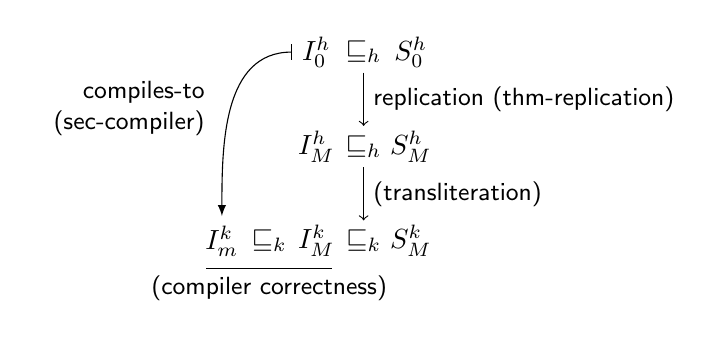
\begin{tikzpicture}
    \node (ih0) at (0, 0) {$I^{h}_{0}$};
    \node (rh0) at (0.6, 0) {$\sqsubseteq_{h}$};
    \node (sh0) at (1.2, 0) {$S^{h}_{0}$};

    \node (ihM) at (0, -1.2) {$I^{h}_{M}$};
    \node (rhM) at (0.6, -1.2) {$\sqsubseteq_{h}$};
    \node (shM) at (1.2, -1.2) {$S^{h}_{M}$};

    \node (ikm) at (-1.2, -2.4) {$I^{k}_{m}$};
    \node (rkm) at (-0.6, -2.4) {$\sqsubseteq_{k}$};
    \node (ikM) at (0, -2.4) {$I^{k}_{M}$};
    \node (rkM) at (0.6, -2.4) {$\sqsubseteq_{k}$};
    \node (skM) at (1.2, -2.4) {$S^{k}_{M}$};

    \draw (-1.4, -2.75) to (0.2, -2.75);
    \node (compCorrect) at (-0.6, -3.0) {\small\sf{(compiler correctness)}};

    \draw[|-{latex}] (ih0) to[out=180,in=90] node[left] {
      \small\sf\begin{tabular}{r}
      compiles-to\\
      (\autoref{sec-compiler})
      \end{tabular}} (ikm);
    \draw[->] (rh0) to node[right] {\small\sf{replication (\autoref{thm-replication})}} (rhM);
    \draw[->] (rhM) to node[right] {\small\sf{(transliteration)}} (rkM);
  \end{tikzpicture}
  \caption{A single-line protocol, a multiline spec, and multiline implementations}
  \label{fig-multiline-spec}
\end{figure}

\autoref{fig-multiline-spec} elaborates more on the role of the multiline specification.
For a given \hemiola{} single-line protocol ($I^{h}_{0}$), we can lift the refinement using the replication theorem to obtain a refinement for the multiline protocol ($I^{h}_{M}$).
Since both \hemiola{} and Kami are rule-based description languages, we expect it is straightforward to have an ideal multiline protocol in Kami ($I^{k}_{M}$) in the sense of simple transliteration, while preserving the refinement.
After all, the correctness of the protocol compiler must be the refinement from a target Kami implementation ($I^{k}_{m}$) to the multiline protocol.
Proving compiler correctness in this manner is on our list of valuable future work.
As already mentioned in \autoref{sec-compiler}, while the compiler may use nontrivial optimizations, they are all within the internal cache design, thus irrelevant to cache-coherence protocol verification.

\end{document}
